% !TeX root = ../../main.tex
\begingroup
\ChFiveBegin
\emergencystretch=2em
\chapter{Temporally annotated longitudinal textual time series from PubMed Open Access clinical case reports}\label{chap:ch05}
\noindent\emph{This chapter is based on:} \cite{noroozizadeh-pmoa-tts-v4}.\par\smallskip

% % !TeX root = ../../../main.tex
\ChFiveAbstract
{
Clinical narratives encode temporal dynamics essential for modeling patient trajectories, yet large-scale temporally annotated resources are scarce. We introduce PMOA-TTS, a corpus of 124{,}349 single-patient PubMed Open Access case reports converted into structured textual timelines of (event, time) pairs using a scalable large-language-model pipeline (\texttt{Llama 3.3 70B} and \texttt{DeepSeek-R1}). The corpus comprises over 5.6 million timestamped events, alongside extracted demographics and diagnoses. Technical validation uses a clinician-curated gold set and three measures: semantic event matching, temporal concordance (c-index), and alignment error summarized with Area Under the Log-Time CDF (AULTC). We benchmark alternative prompting and model choices and provide documentation to support reproduction. 
\ChFiveRebuttal{
PMOA-TTS provides a large, publicly available resource for developing and evaluating methods for clinical timeline extraction and temporal reasoning from narrative text.
}
% PMOA–TTS enables research on timeline extraction, temporal reasoning, survival modeling and event forecasting from narrative text, and offers broad diagnostic and demographic coverage. 
Data and code are openly available in public repositories.
% PMOA–TTS dataset is hosted on Hugging Face Datasets at \url{https://huggingface.co/datasets/snoroozi/pmoa-tts}. Our full codebase, including preprocessing scripts, prompt templates, and evaluation pipelines,
% is available at: \url{https://github.com/jcweiss2/pmoa_tts}. 
}.

%\ChFiveKeywords{keyword1, Keyword2, Keyword3, Keyword4}
\ChFiveKeywords{clinical natural language processing, temporal information extraction, textual time series, large language models, PubMed Open Access case reports}



% Background & Summary
% Methods
% Data Records
% Data Overview (optional)
% Technical Validation
% Usage Notes (optional)
% Data Availability
% Code Availability
% References
% Author Contributions
% Competing Interests
% Acknowledgements (optional)
% Funding
% Ethics statement* 

%%%%%%%%%%%%%%%%%%%%%%%%%%%%%%%%%%%%%%%%%%%%%%
%%%%%%%%%%%%%% Introduction %%%%%%%%%%%%%%%%%
%%%%%%%%%%%%%%%%%%%%%%%%%%%%%%%%%%%%%%%%%%%%%

% !TeX root = ../../../main.tex
\subsection{Introduction}
\label{ch05:sec:introduction}

Understanding when clinical events occur is fundamental to modeling patient trajectories, enabling tasks such as process mining, outcome forecasting, and causal inference in medicine \citep{jensen2012mining,noren2010temporal,noroozizadeh2025forecasting}.
\ChFiveRebuttal{
Although a case report is a dated document, it does not provide a machine-readable timestamp for each clinical event. Event times are instead expressed within the narrative through relative, coarse, or implicit phrases. PMOA-TTS converts these mentions into normalized event-time tuples for longitudinal analysis.
}
While electronic health record (EHR) datasets like MIMIC-III and MIMIC-IV include timestamped structured data and clinical notes \citep{johnson2016mimic,ch05:johnson2023mimic}, they capture only a subset of events (e.g., vital signs, lab results) and still require sophisticated natural language processing to extract temporal information from unstructured text \citep{viani2021temporal,cheng2023typed}.


In contrast, published case reports often provide rich narrative descriptions of patient timelines, but the timing of events is typically expressed in relative terms within the free text (e.g., “on day 3 of hospitalization”).
Efforts in temporal reasoning on clinical text have been hampered by the scarcity of large-scale annotated corpora.
Earlier initiatives, such as the 2012 i2b2 challenge and Clinical TempEval, focused on temporal relation extraction from clinical notes \citep{sun2013evaluating,bethard2016semeval,galvan2018investigating} but were constrained by small datasets (e.g., 310 documents) from single institutions, limiting model performance and generalizability.
Systems that rely on metadata timestamps (e.g., admission or discharge dates) fail to capture the fine-grained sequence of clinical events described in text, which is essential for nuanced understanding and prediction.
There remains a pressing need for large-scale, temporally annotated corpora to support the development and evaluation of models for clinical temporal reasoning.

\ChFiveRebuttal{
We selected PMC Open Access case reports because they are publicly accessible, clinically detailed narratives that often connect pre-presentation history, diagnostic work-up, treatment rationale, hospitalization, and follow-up within a single document. Their enrichment for rare and atypical presentations provides a demanding setting for temporal extraction, but PMOA-TTS should not be interpreted as a population-representative cohort.
}


Building on our pilot pipeline on 10 case reports \citep{wang2025large}, we introduce the PubMed Open Access Textual Time Series (PMOA–TTS) corpus—a large-scale dataset of 124{,}349 openly available clinical case reports, each annotated with a structured timeline of events.
Leveraging large language models (LLMs)—specifically \texttt{Llama 3.3 70B} \citep{grattafiori2024llama} and \texttt{DeepSeek-R1} \citep{guo2025deepseek}—we transform each case report into a sequence of \mbox{(clinical event, time)} tuples that capture key clinical events and their relative timing within the patient narrative (Figure \ref{ch05:fig:annotation_ex}).
To the best of our knowledge, PMOA–TTS constitutes the largest publicly available collection of clinical narratives with explicit temporal event structure.
Compared to our prior pilot study \cite{wang2025large}, we expand the manually annotated reference set from 10 to 200 case reports and scale the LLM-annotated timelines from 100 to 124{,}349 reports. 

Building PMOA-TTS requires addressing three challenges at scale: reliably identifying single-patient case reports, extracting timeline events with high fidelity from ambiguous free-text expressions, and rigorously evaluating the resulting annotations.
We meet these needs with an LLM-based pipeline that selects relevant narratives beyond metadata filters, resolves relative time language into fine-grained event--time tuples, and enriches each case with structured demographics and diagnoses. 


% !TeX root = ../../../main.tex
\begin{figure}[htbp]
\begin{ChFiveFloatBody}

  \centering

  \subfloat[{Case narrative with highlighted clinical events}]{\begin{minipage}[t]{0.49\textwidth}
    \begin{tcolorbox}
    [
    colback=white,
    colframe=black!30,
    arc=2mm,
    boxrule=0.6pt,
    left=2mm,right=2mm,top=2mm,bottom=2mm
    ]
      \small\raggedright
      A \hl{52-year-old} \hl{woman} was \hl{admitted to the medical ICU} with \hl{chest pain} and \hl{shortness of breath}. She developed \hl{intermittent fever and fatigue} a couple of weeks prior to admission. Eight hours after hospital and ICU admission, \hl{broad-spectrum antibiotics} were \hl{started for suspected infection}. On hospital admission day 2, she developed \hl{pleuritic pain} and \hl{escalating oxygen requirements}. \hl{CT angiography} was performed two days after admission.
      
    \end{tcolorbox}
    
    \label{ch05:fig:narrative_box}
  \end{minipage}}\hfill%
  \subfloat[{Text-ordered event–time tuples.}]{\begin{minipage}[t]{0.49\textwidth}
    \begin{tcolorbox}
    [
    colback=white,
    colframe=black!30,
    arc=2mm,
    boxrule=0.6pt,
    left=2mm,right=2mm,top=2mm,bottom=2mm
    ]
      \small\centering
      \setlength{\tabcolsep}{5pt}
      \begin{adjustbox}{max width=\linewidth}\begin{tabular}{@{} l r @{}}
        \toprule
        \textbf{Event} & \textbf{Time (h)} \\
        \midrule
        52-year-old & 0 \\
        woman & 0 \\
        admitted to the medical ICU & 0 \\
        chest pain & 0 \\
        shortness of breath & 0 \\
        developed intermittent fever & -336 \\
        developed fatigue & -336 \\
        broad-spectrum antibiotics started \\ for suspected infection & 8 \\
        pleuritic pain developed & 24 \\
        escalating oxygen requirements & 24 \\
        CT angiography & 48 \\
        %Management decisions & 48 \\
        \bottomrule
      \end{tabular}\end{adjustbox}
    \end{tcolorbox}
    
    \label{ch05:fig:table_box}
  \end{minipage}}

  
  
  

\end{ChFiveFloatBody}
\caption{Example case report (left) with text-ordered event-time tuples (right).
  }\ChFiveFloatLabel{ch05:fig:annotation_ex}
\end{figure}






\ChFiveRebuttal{
In summary, we (i) introduce the PMOA Textual Time Series (PMOA-TTS) corpus of 124{,}349 single-patient case reports from PubMed Open Access, each annotated with structured clinical timelines extracted using large language models; (ii) develop a scalable pipeline for automatic case identification and prompt-driven extraction of timelines, demographics, and diagnoses, together with a manual evaluation framework; (iii) define and apply complementary validation measures for timeline accuracy, including temporal order concordance (c-index) and the Area Under the Log-Time CDF (AULTC); and (iv) characterize corpus properties (demographics, frequent diagnoses, and co-occurrence structure) to document clinical and demographic breadth.
}

PMOA–TTS offers several contributions to the biomedical NLP and clinical AI communities.
By releasing the largest openly available dataset of temporally structured clinical narratives, this work democratizes access to timeline-based clinical text—an area typically limited to proprietary EHR datasets.
The corpus spans a wide range of diagnoses and demographics, supporting research on temporal patterns in diverse and sometimes underrepresented conditions.
By making the extraction pipeline, prompting strategies, and evaluation framework publicly available, the project promotes transparency and reproducibility in LLM-based clinical information extraction.
These contributions collectively advance the development of models for timeline reconstruction, temporal reasoning, and longitudinal prediction, while lowering the barrier
to entry for researchers working in resource-limited settings.




% !TeX root = ../../../main.tex
\subsection{Methods}
\label{ch05:sec:methods}

Our pipeline comprises the following key components: dataset extraction, textual time series annotation, and comprehensive evaluation of the annotations (Figure~\ref{ch05:fig:flowchart}).


% !TeX root = ../../../main.tex
\begin{figure}[htbp]
\begin{ChFiveFloatBody}
 % 'r' for right, 'l' for left
    \centering
    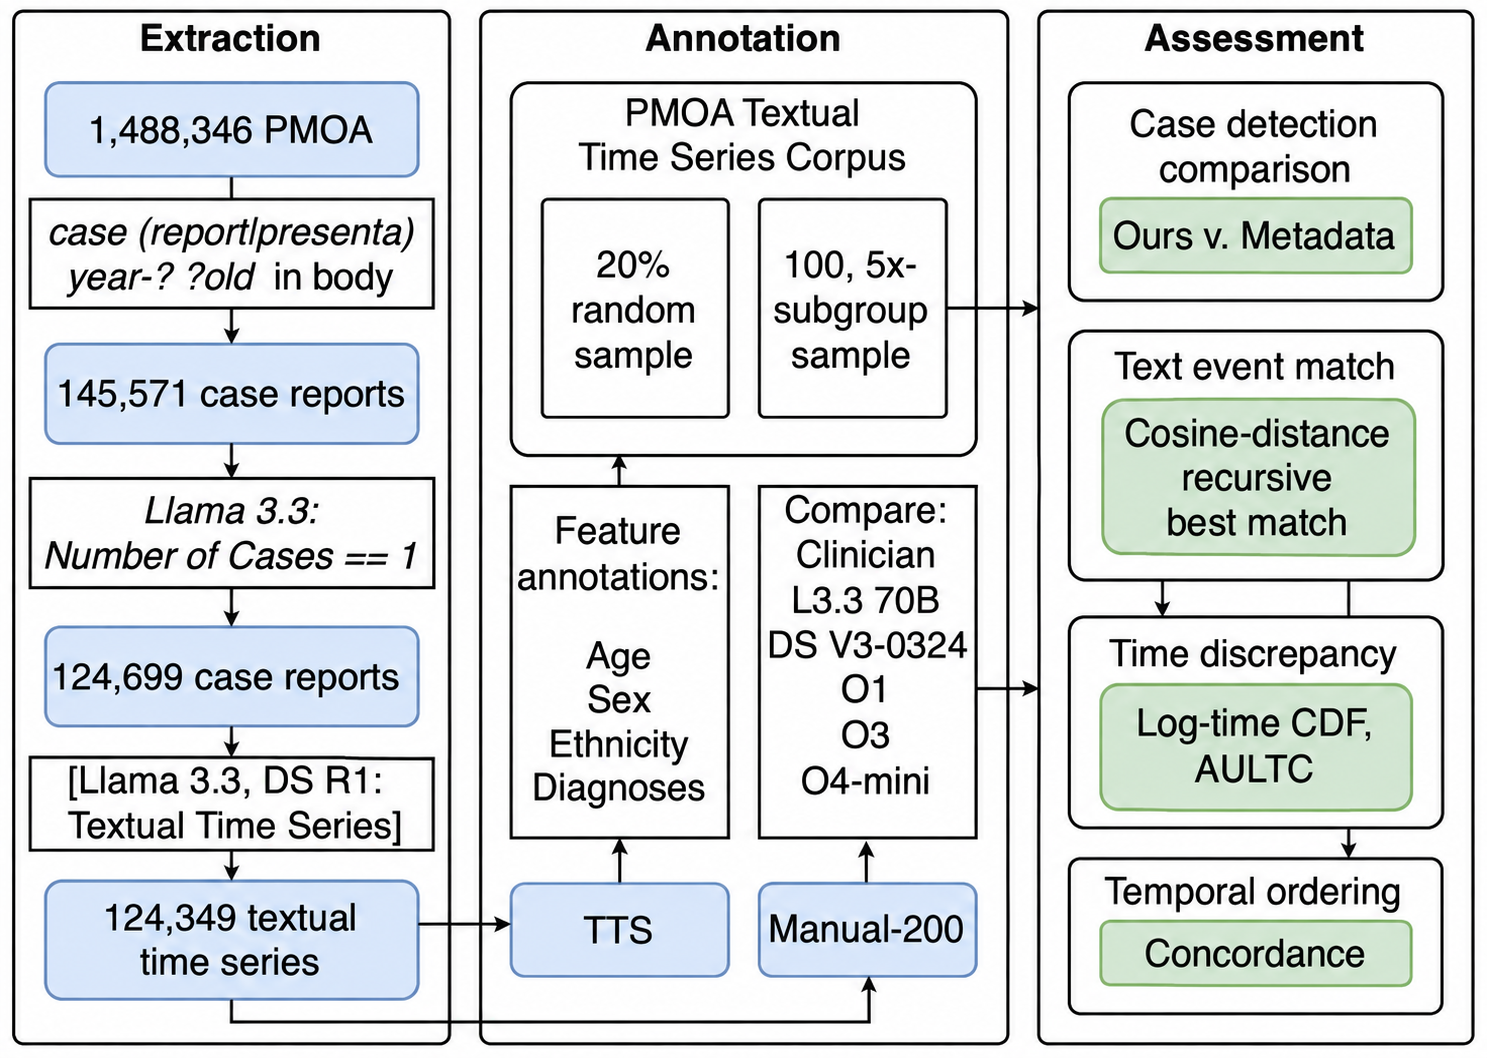
\includegraphics[width=0.75\linewidth]{Chapters/chapter-05/images/Scientific_data/Plots_tables/PMOATTS_flow5_v2.png} % Adjust width
    
    
    

\end{ChFiveFloatBody}
\caption{Flowchart of the extraction and annotation pipeline. The left panel (Extraction) shows how we filtered the PMOA corpus to identify single-patient case reports. The middle panel (Annotation) depicts the generation of textual time series for each case via LLM prompting and the creation of evaluation subsets. The right panel (Assessment) summarizes the evaluation process, including metadata comparison, text event matching, time discrepancy analysis (log-time CDF, AULTC), and temporal order concordance.
    }\ChFiveFloatLabel{ch05:fig:flowchart}
\end{figure}



% !TeX root = ../../../main.tex
\begingroup\raggedright
\subsubsection{Case Report Identification Pipeline}
\label{ch05:sec:case-report-identification-pipeline}

\ChFiveRebuttal{
We obtained the source corpus from the PubMed Central Open Access Subset using the NCBI FTP bulk-download service available at the time of collection. Specifically, we used the 12 plain-text baseline archives in \texttt{oa\_bulk/oa\_noncomm/txt} dated 17 December 2024, with filenames ranging from \texttt{oa\_noncomm\_txt.PMC000xxxxxx.baseline.2024-12-17.tar.gz} to \texttt{oa\_noncomm\_txt.PMC011xxxxxx.baseline.2024-12-17.tar.gz}, downloaded from the then-current endpoint \url{https://ftp.ncbi.nlm.nih.gov/pub/pmc/oa_bulk/oa_noncomm/txt/}. After unpacking the archives, we extracted article content between the ``\texttt{==== Body}'' and ``\texttt{==== Ref}'' markers. Candidate reports were identified using the case-insensitive regular expressions \texttt{case (report|presenta)} and \texttt{year-? ?old}. We then retained documents for which \texttt{Llama 3.3 70B Instruct} returned \texttt{1} to the single-patient case-count prompt. Each released record retains its source PMCID.
}

\ChFiveRebuttal{
The source files were drawn from the non-commercial-use collection of the PMC Open Access Subset. Reuse conditions vary by article and are governed by the license statement attached to each source article; the source PMCID is retained for every PMOA-TTS record to preserve provenance and license traceability.
}

This filter yields 145,571 candidate documents likely to be case reports or case series. 
\ChFiveRebuttal{
The regular expressions serve as deterministic candidate-generation criteria that define the document pool considered for corpus construction; PMOA-TTS does not claim exhaustive retrieval of every possible single-patient case report in PMOA.
}
For the single-patient case-count step, the model is prompted with: ``\texttt{You are a physician. Determine the number of case reports in the following manuscript. Return 0 if it is not a case report. Reply only with the number and nothing else.}'', followed by the document body.
\ChFiveRebuttal{
The pipeline selected 124{,}699 source articles as single-patient case reports. Of these, 124{,}349 produced valid event-time rows. 350 outputs were excluded because they could not be parsed into the required schema.
}
This two-stage process results in a final dataset of \ChFiveRebuttal{124{,}349} single-patient case reports (Figure~\ref{ch05:fig:flowchart}).

We compared our LLM-based case report identification method with PubMed's metadata-based labeling using a carefully designed benchmark.
We created a dataset of 100 reports across five diagnoses—Diabetes, Sepsis, Hypertension, COVID-19, and Atrial Fibrillation—with 10 reports per diagnosis from each method.
A clinician manually reviewed and labeled each report to verify whether it described exactly one case.
\ChFiveRebuttal{
Because this evaluation set was constructed from documents surfaced by at least one of the two identification approaches, recall is computed with respect to manually confirmed single-patient case reports within this evaluation set and should not be interpreted as corpus-level sensitivity over all PMOA documents.
}


%%%%%%%%%%%%%%%%%%%%%%%%%%%%
%%%%%%%%%%%%%%%%%%%%%%%%%%%%

\par\endgroup

% !TeX root = ../../../main.tex
\subsubsection{Timeline Annotation via LLM Prompting}
\label{ch05:sec:timeline-annotation}

\ChFiveHeadingOnly
\paragraph{Textual Time Series (TTS)}
\label{ch05:sec:textual-time-series}

We use large language models (LLMs; \texttt{LLaMA\~3.3\~70B}, \texttt{DeepSeek-R1}) to convert PubMed Open Access (PMOA) case reports into \emph{textual time series} (TTS).
A textual time series is defined as an ordered sequence of clinical event–time pairs, where each event is represented as a short free-text span and each timestamp is a numeric value measured in hours relative to a case-specific reference time.
\ChFiveRebuttal{
The reference event is an anchor for the timeline rather than its boundary. For the LLM extraction, hospital admission is assigned $t=0$ when it is described. If admission is not described, the current clinical presentation that frames the case, such as the main diagnosis or treatment, is assigned $t=0$. Events before and after this reference event receive negative and positive timestamps, respectively. Thus, a phrase such as ``three days before admission'' is represented as $-72$ hours, whereas an event on hospital day 2 is represented as $+24$ hours. Depending on the source report, the resulting TTS may cover an acute encounter or a longitudinal course extending over months or years.
}

In this work, a clinical event refers to any health-related mention that can stand alone semantically and is directly relevant to the patient’s course.
This includes symptoms and signs, diagnoses, procedures and diagnostic tests, treatments and medication administrations, major clinical states, and outcomes.
Explicitly stated pertinent negatives and termination events (such as “no shortness of breath” or “antibiotics discontinued”) are also included. 
Demographic attributes that appear in the narrative, such as age and sex are also extracted as clinical events with reference time (t=0) as the timestamp.
We exclude purely contextual text that does not describe the index patient, such as general background statements or literature discussion.


\ChFiveRebuttal{
PMOA-TTS uses source-faithful, span-based events in the tradition of i2b2 clinical concept annotation, while allowing enough surrounding context for an event to remain clinically interpretable, in contrast to span-based temporal annotation methods (e.g., \cite{sun2013evaluating,uzuner20112010}) and i2b2-style guidelines that often limit events to short prepositional phrases. This is necessary because the timelines include symptoms, findings, procedures, treatments, outcomes, pertinent negatives, uncertainty, and intent in addition to diagnoses. For example, retaining ``pain in chest that radiates substernally'' preserves information that would be lost if the event were reduced to a generic chest-pain code; similarly, retaining ``planned'' distinguishes an intended procedure from one that occurred.
}
Conjunctive mentions are separated into individual events when doing so improves clarity.

Natural-language time expressions are normalized into hour units: coarse expressions such as “hospital day 2” are converted using 24-hour increments from the reference point, interval expressions are represented using the start of the interval, and vague temporal phrases are resolved to approximate offsets that are consistent with narrative ordering and surrounding cues.
The goal of this normalization is to produce a usable relative timeline rather than an exact reconstruction of clock time.

The above specifications define the intended representation of textual time series.
The LLM extraction prompt used in our pipeline (Supplementary Material, Section~\ref{ch05:apd:extraction-prompt}) implements this specification by instructing the model to output a structured sequence of \mbox{(clinical event, time)} tuples.
Events are kept in free-text form to retain clinical specificity rather than being normalized to a fixed ontology.
On average, each case report yields 46 events, and the full corpus comprises over 5.6 million timestamped events, making it the largest publicly available resource of this type in clinical NLP.


\paragraph{Gold Standard Annotations}
\label{ch05:sec:gold-standard-annotations}

We constructed a gold-standard reference set of 200 manually annotated case reports, consisting of 190 cases randomly sampled from PMOA–TTS and 10 cases from our prior pilot study.
All annotations were performed by a single clinical expert following a detailed annotation guideline designed to preserve fidelity to the original narrative while producing event representations suitable for temporal evaluation.

Annotators marked exact text spans corresponding to clinical events without rewriting or paraphrasing, with a small number of controlled exceptions specified in the guideline.
First, conjunctive findings (e.g., “nausea and vomiting”) were permitted to be split into individual events when clinically meaningful.
Second, when needed to supply context, annotators could prepend short clarifying phrases such as “history of” to ensure that extracted events were interpretable as stand-alone findings.
Beyond these two exceptions, events were expected to remain faithful to the wording and granularity of the source text.

To promote consistency, annotators were then instructed to ensure that each event was semantically self-contained (e.g., using “SCC of the lung” rather than “SCC” to avoid ambiguity with other
entities such as cutaneous squamous cell carcinoma or sickle cell crisis).
Related findings were disambiguated when necessary, duplicate mentions of the same event were avoided even when they appeared in multiple sections of a report, and pertinent negative or termination events (e.g., “no shortness of breath” or “denies chest pain”) were included when explicitly stated.
These conventions were applied uniformly across all 200 annotated case reports.

Each annotated event was assigned a timestamp relative to a standardized case reference point.
By definition, this reference point was the time of admission.
If an explicit admission time was not stated, the encounter date (the earliest unambiguous point of primary clinical evaluation within the case narrative) was used as the reference time.
For temporal expressions that described intervals, the start time of the interval was recorded.
All timestamps were expressed in hours relative to the reference time (t=0).

These manually produced timelines serve as the reference standard for evaluating LLM-generated annotations in subsequent sections.


% !TeX root = ../../../main.tex
\subsubsection{Evaluation Metrics}
\label{ch05:sec:evaluation-metrics}

We next assessed the quality of the extracted textual time series using the 200 manually annotated case reports as reference.
Each large language model (LLM) annotator was evaluated across five independent runs to capture run-to-run variation in the generated timelines.
For each model and run, we computed three complementary metrics as described below (detailed description in Supplementary Material, Section \ref{ch05:apd:evaluation-metrics}).

\ChFiveParagraph{Event match rate (recall, precision, and F1)}

To evaluate alignment between predicted and reference clinical events, we applied a recursive best-match strategy adapted from prior work \citep{wang2025large,pmlr-v333-noroozizadeh26a}, as summarized in Algorithm~\ref{ch05:alg:recursive_match}.
At each iteration, the method selects the closest unmatched predicted--reference pair under a text-similarity metric, retains the match if it falls below a distance threshold, and removes both events before continuing.
This procedure yields an efficient one-to-one alignment that accommodates timelines of unequal length.

\ChFiveRebuttal{
We evaluate event identification using event match recall, precision, and F1. Let $M$ denote the number of one-to-one semantic matches after assignment and application of the cosine-distance threshold, $N_{\mathrm{manual}}$ the number of manually annotated events, and $N_{\mathrm{model}}$ the number of model-generated events. Event match recall is defined as $M/N_{\mathrm{manual}}$, event match precision as $M/N_{\mathrm{model}}$, and event match F1 as the harmonic mean of precision and recall. Precision therefore penalizes additional model-generated events that remain unmatched under the one-to-one alignment, complementing recall, which measures the proportion of manually annotated events recovered.
}

As a sensitivity analysis, we also evaluated a globally optimal one-to-one alignment based on the Linear Assignment Problem (LAPJV) \citep{jonker1987shortest}.
Across all models, results differed by at most $0.3$ percentage points in event match recall relative to the recursive heuristic.
We therefore report results using the recursive matching strategy in the main text and provide full LAPJV details and comparison tables in the Supplementary Material (Section~\ref{ch05:apd:lapjv-matching}).


\ChFiveParagraph{Temporal metrics}

We used 2 metrics which evaluate how well the LLM extracts timestamps of clinical events: (a) \textbf{\emph{Temporal concordance}} (c-index) evaluates whether the relative ordering of event times in the model output agrees with the manually annotated timelines, providing an order-based summary of temporal consistency. (b) \textbf{\emph{Log-time discrepancy}} quantifies the absolute difference between the log-transformed timestamps of matched events, and we summarized its distribution using the Area Under the Log-Time CDF (AULTC), which captures the cumulative proportion of events achieving small timing errors. \ChFiveRebuttal{
AULTC is computed over semantically matched event pairs only and therefore measures timestamp accuracy conditional on successful event alignment. Unmatched events do not enter the empirical CDF or AULTC and are evaluated separately by the event-extraction metrics. 
}




% !TeX root = ../../../main.tex
\subsection{Data Records}
\label{ch05:sec:data-records}

\ChFiveRebuttal{
The PMOA-TTS dataset is deposited on Hugging Face \cite{shahriar_noroozizadeh_2026} and is publicly available at \url{https://doi.org/10.57967/hf/10546}.
}
\ChFiveRebuttal{
PMOA-TTS distributes derived structured annotations and source identifiers rather than copies of source-article text, figures, images, or supplementary files. The released annotations and metadata are licensed under CC BY-NC-SA 4.0 (\url{https://creativecommons.org/licenses/by-nc-sa/4.0/}); reuse of the underlying source articles remains subject to the article-level terms displayed by PMC (\url{https://pmc.ncbi.nlm.nih.gov/tools/openftlist/}).
}
The dataset card lists task tags (\texttt{Text Classification}), modality (\texttt{Text}), format support (\texttt{Parquet via auto-conversion}), language (\texttt{English}), and size (``\texttt{100K--1M}'').
Data record schema with an example JSON entry is shown in Figure~\ref{ch05:fig:record_schema}.
% \ChFiveRebuttal{
% The demographic fields are LLM-extracted or LLM-mapped descriptors from the case-report narrative. They should not be interpreted as independently verified biological sex at birth, self-identified race or ethnicity, or population-representative demographic measurements. The model returns Not Specified when no value is identified; ethnicity is Not Specified in 89\% of reports.
% }

\noindent PMOA-TTS has the following dataset splits:

% !TeX root = ../../../main.tex
\begin{figure}[htbp]
\begin{ChFiveFloatBody}

\centering

\begin{minipage}[t]{1\textwidth}
\centering
\footnotesize
\begin{adjustbox}{max width=\linewidth}\begin{tabular}{@{} l l >{\raggedright\arraybackslash}p{4cm} @{}}
\toprule
\textbf{Field} & \textbf{Type} & \textbf{Description} \\
\midrule
\texttt{pmc\_id} & str &
Folder-level ID (PMC000xxxxxx--PMC011xxxxxx). \\

\texttt{case\_report\_id} & str &
Filename of the case (e.g., PMC6417290). \\

\texttt{textual\_timeseries} & List[Dict] &
Sequence of \{"event": str, "time": int\}. \\

\texttt{demographics} & Dict &
\{"age": str/"Not Specified", "sex": str, "ethnicity": str\}. \\

\texttt{diagnoses} & List[str] &
List of diagnosis terms extracted per case. \\

\bottomrule
\end{tabular}\end{adjustbox}
\end{minipage}
\hfill

\begin{minipage}[t]{\linewidth}
\centering
\begin{tcolorbox}[
  colback=gray!5,
  colframe=gray!70,
  title=Example JSON entry,
  boxrule=1pt,
  enhanced,
  %breakable,
  fontupper=\footnotesize
]
\begin{verbatim}
"pmc_id": "PMC006xxxxxx",
"case_report_id": "PMC6417290",

"textual_timeseries": [
  {"event": "56 years old", "time": 0},
  {"event": "male", "time": 0},
  {"event": "HIV-positive", "time": 0},
  {"event": "admitted to the hospital", "time": 0},
  {"event": "knee arthralgia", "time": 0},
  ...
  {"event": "postural headache", "time": 48},
  {"event": "neurological examination", "time": 120},
  {"event": "persistence of headache", "time": 144},
  {"event": "brain computed tomography scan",
   "time": 144},
  ...
  {"event": "symptom free", "time": 4320},
  {"event": "CT scan", "time": 4320},
  {"event": "no brain shift", "time": 4320}
],
"diagnoses": [
  "HIV",
  "Knee arthralgia",
  "Subdural hematoma",
  "Postdural puncture headache (PDPH)"
],
"demographics": {
  "age": 56,
  "sex": "Male",
  "ethnicity": "Not Specified"
}
\end{verbatim}
\end{tcolorbox}
\end{minipage}





\end{ChFiveFloatBody}
\caption{\textbf{top:} PMOA-TTS record schema. \textbf{bottom:} compact example matching the schema above (drawn from our HuggingFace repository (formatted for readability).}\ChFiveFloatLabel{ch05:fig:record_schema}
\end{figure}




\begin{itemize}
    \item \texttt{train\_DSR1/L33}: The full TTS release contains \ChFiveRebuttal{124{,}349 records} with valid event-time rows.
The \texttt{train\_DSR1} and \texttt{train\_L33} splits contain annotations generated using \texttt{DeepSeek-R1} and \texttt{Llama 3.3 70B}, respectively.
Here, a split denotes a version of the dataset defined by the annotation model used.
These splits serve as the default releases and contain the primary annotations used in downstream analyses.
    
    \item {\raggedright \ChFiveRebuttal{\texttt{case\_study\_100} contains the TTS-bearing portion of the 100-document case-identification evaluation. Of the 100 candidate documents reviewed, 88 were confirmed to contain a single-patient case report and therefore have TTS annotations; the remaining 12 did not contain a case report and consequently have no patient timeline in this split.}\par}
    
    \item \texttt{case\_study\_n200}: A benchmark of 200 manually reviewed case reports used for qualitative and quantitative evaluation of LLM-generated annotations.
Each model is evaluated across five independent runs on this subset to assess run-to-run variability in annotation consistency.

\end{itemize}

The data repository also has an additional data split \texttt{TTS\_n200\_additional\_models}, which bundles the single-expert manual timelines (the reference set) together with parallel LLM-generated textual time series for additional models, including open-weight models such as \texttt{DeepSeek-V3}, \texttt{DeepSeek-R1 quantized}, and \texttt{DeepSeek-V3-0324}, and proprietary OpenAI models such as \texttt{GPT5}, \texttt{O1}, \texttt{O3}, and \texttt{O4-mini}.
This split is designed for lightweight benchmarking and cross-model comparison on a fixed 200-case cohort without re-annotating the full corpus.
For the full \ChFiveRebuttal{124{,}349} release, we provide textual time series produced by \texttt{DeepSeek-R1} and \texttt{Llama 3.3 70B}; the additional models are released only on the 200-case subset due to resource constraints.
For completeness, both \texttt{Llama 3.3 70B} and \texttt{DeepSeek-R1} were also executed in five independent runs on the \texttt{case\_study\_n200} subset, and these annotated outputs are included in the dataset.
\ChFiveRebuttal{Additional details regarding exact model versions, access dates, decoding settings, context limits, seeds, and the inference framework are available in Supplementary Material Section  \ref{ch05:sec:supp-model-configuration}}.


% !TeX root = ../../../main.tex
\ChFiveStarSubsection{Data Availability}
\ChFiveRebuttal{
The PMOA-TTS dataset is publicly available on Hugging Face at \url{https://huggingface.co/datasets/snoroozi/pmoa-tts} under the CC BY-NC-SA 4.0 license. The version of record cited in this article is available at \url{https://doi.org/10.57967/hf/10546}. The code used for corpus construction and technical validation is available at \url{https://github.com/jcweiss2/pmoa_tts}.
}



% !TeX root = ../../../main.tex
\ChFiveStarSubsection{Ethics Statement}
% \label{sec:ethics-statement}
\ChFiveRebuttal{
This study is a secondary analysis of publicly available, previously published case reports from the PubMed Central Open Access Subset. No participants were recruited and no non-public clinical records were accessed. The released dataset contains derived structured annotations and source PMCIDs rather than copies of the source articles.
}

%%%%%%%%%%%%%%%%%%%%%%%%%%%%%%%%%%%%%%%%%
%%%%%%%%%%%%%%%% Data Overview
%%%%%%%%%%%%%%%%%%%%%%%%%%%%%%%%%%%%%%%%


% !TeX root = ../../../main.tex
\subsection{Data Overview}
\label{ch05:sec:data-overview}


% !TeX root = ../../../main.tex
\ChFiveHeadingOnly
\subsubsection{Cohort Demographics}
\label{ch05:sec:cohort-demographics}

For demographic extraction, we used an LLM-based query to retrieve age, sex, and ethnicity for each case.
The prompt instructed the model to report age in years; sex as \texttt{Male}, \texttt{Female}, a free-text category, or \texttt{Not Specified}; and ethnicity according to U.S.\ Census categories or \texttt{Not Specified} (full prompt in Supplementary Material, Section~\ref{ch05:apd:demographics-prompt}).
\ChFiveRebuttal{
The demographic fields are LLM-extracted or LLM-mapped descriptors from the case-report narrative. They should not be interpreted as independently verified biological sex at birth, self-identified race or ethnicity, or population-representative demographic measurements.
}

Across PMOA-TTS, the median age is 47 years, with peaks at 5-year intervals, consistent with rounded age reporting in clinical text (Figure~\ref{ch05:fig:demo}).
The distribution of LLM-extracted sex descriptors is approximately balanced (52\% male, 47\% female, 1\% Not Specified).
\ChFiveRebuttal{
Ethnicity was not specified in 89\% of reports. Among reports with an extracted ethnicity category, White/Caucasian and Asian were the most frequent. Given the extensive missingness and the non-population-based nature of case reports, these proportions should not be interpreted as population prevalence or attributed to a specific underlying cause.
}


% !TeX root = ../../../main.tex
\begin{figure}[htbp]
\begin{ChFiveFloatBody}

  \centering
  \begin{minipage}[t]{0.49\linewidth}
    \centering
    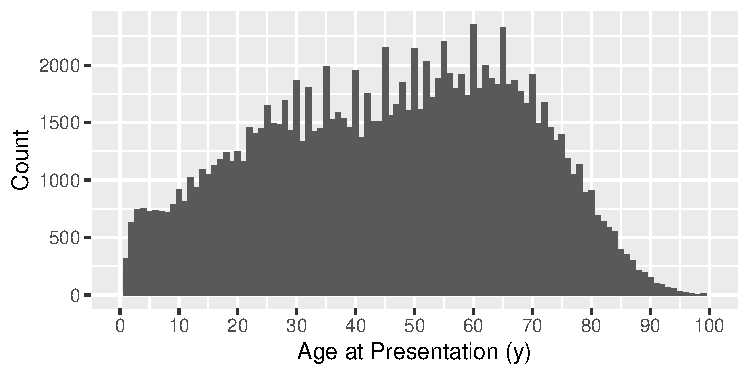
\includegraphics[width=\linewidth]{Chapters/chapter-05/images/Scientific_data/Plots_tables/125k_age.pdf}
  \end{minipage}\hfill
  \begin{minipage}[t]{0.49\linewidth}
    \centering
    \scriptsize
    \begin{tabular}{l r}
      \toprule
      \textbf{Characteristic} & \textbf{Percent (\%)}\\
      \midrule
      \multicolumn{2}{l}{\textbf{Sex}}\\
      \quad Male & 52\\
      \quad Female & 47\\
      \quad Not Specified & 1\\
      \midrule
      \multicolumn{2}{l}{\textbf{Ethnicity}}\\
      \quad White/Caucasian & 5\\
      \quad Asian & 3\\
      \quad African & 1\\
      \quad Other & 2\\
      \quad Not Specified & 89\\
      \bottomrule
    \end{tabular}
  \end{minipage}
  
  
  

\end{ChFiveFloatBody}
\caption{\ChFiveRebuttal{Age distribution and LLM-mapped/extracted demographic descriptors for 124{,}349 PMOA-TTS case reports.}}\ChFiveFloatLabel{ch05:fig:demo}
\end{figure}




% !TeX root = ../../../main.tex
\subsubsection{Descriptive Statistics}
\label{ch05:sec:descriptive-statistics}

The textual time series (TTS) derived from case reports show substantial variation in sequence length and temporal span. 
On average, each TTS contains $46$ timesteps (mean) %\jeremy{mean? median?}, 
with 50\% of sequences comprising between 33 and 57 timesteps (Figure~\ref{ch05:fig:tts_stats}a). 
The length distribution is right-skewed, with a small number of very long trajectories exceeding $1{,}000$ timesteps. 
Events are generally concise: the mean event span is 3.6 words (26.1 characters), and most events fall between two and five words, such as \texttt{“admitted to the hospital”} or \texttt{“CT scan performed”}. 
Longer spans (e.g., $\geq 15$ words) typically correspond to detailed histopathologic or imaging descriptions.

Figure~\ref{ch05:fig:tts_stats}b summarizes the most frequent event strings across the corpus and reflects commonly documented demographic descriptors and clinical milestones (e.g., \texttt{``male''}, \texttt{``female''}, \texttt{``admitted to the hospital''}, \texttt{``discharged''}), as well as prevalent conditions and symptoms (e.g., \texttt{``hypertension''}, \texttt{``fever''}, \texttt{``vomiting''}). 
Importantly, these counts are computed from the \emph{event strings in the TTS} and therefore capture only information that is explicitly stated and extracted as an event in the narrative. 
\ChFiveRebuttal{The demographic percentages in Section~\ref{ch05:sec:cohort-demographics} are patient-level outputs from the dedicated demographic extraction, with one demographic record per report. In contrast, Figure \ref{ch05:fig:tts_stats}b counts literal event strings in the TTS - 57,394 occurrences of male and 52,437 occurrences of female, which do not sum to the total number of case reports in our corpus (n = 124,349). This is because some reports ($14\%$) do not explicitly state sex in a way that is extracted as an event.}
% As a result, demographic events such as \texttt{``male''} and \texttt{``female''} need not sum to the total number of case reports (124k), because some reports ($14\%$) do not explicitly state sex in a way that is extracted as an event.
%even when a separate demographic field may be populated by an auxiliary extraction step.


The temporal coverage of individual case reports also varies widely. 
The mean case duration is 415.9 days (median 104.0 days), with half of cases spanning between 28 and 391 days and the 99th percentile extending to 4{,}380 days (12 years). 
On average, 77.6\% of events share timestamps with at least one other event, indicating frequent temporal co-occurrence within a report. 
The median uniqueness ratio of event timestamps is 0.14, reflecting the common practice of documenting multiple events at the same recorded time (e.g., grouped laboratory results or procedure bundles). 
Approximately 17\% of events have negative timestamps, representing history prior to the chosen reference point (typically admission), such as past diagnoses or prior treatments.
Together, these statistics summarize the density and temporal heterogeneity of clinical event sequences across PMOA-TTS. 

% \vspace{-5mm}

% !TeX root = ../../../main.tex
\begin{figure}[htbp]
\begin{ChFiveFloatBody}

    \centering
    \begin{minipage}{0.48\textwidth}
        \centering
        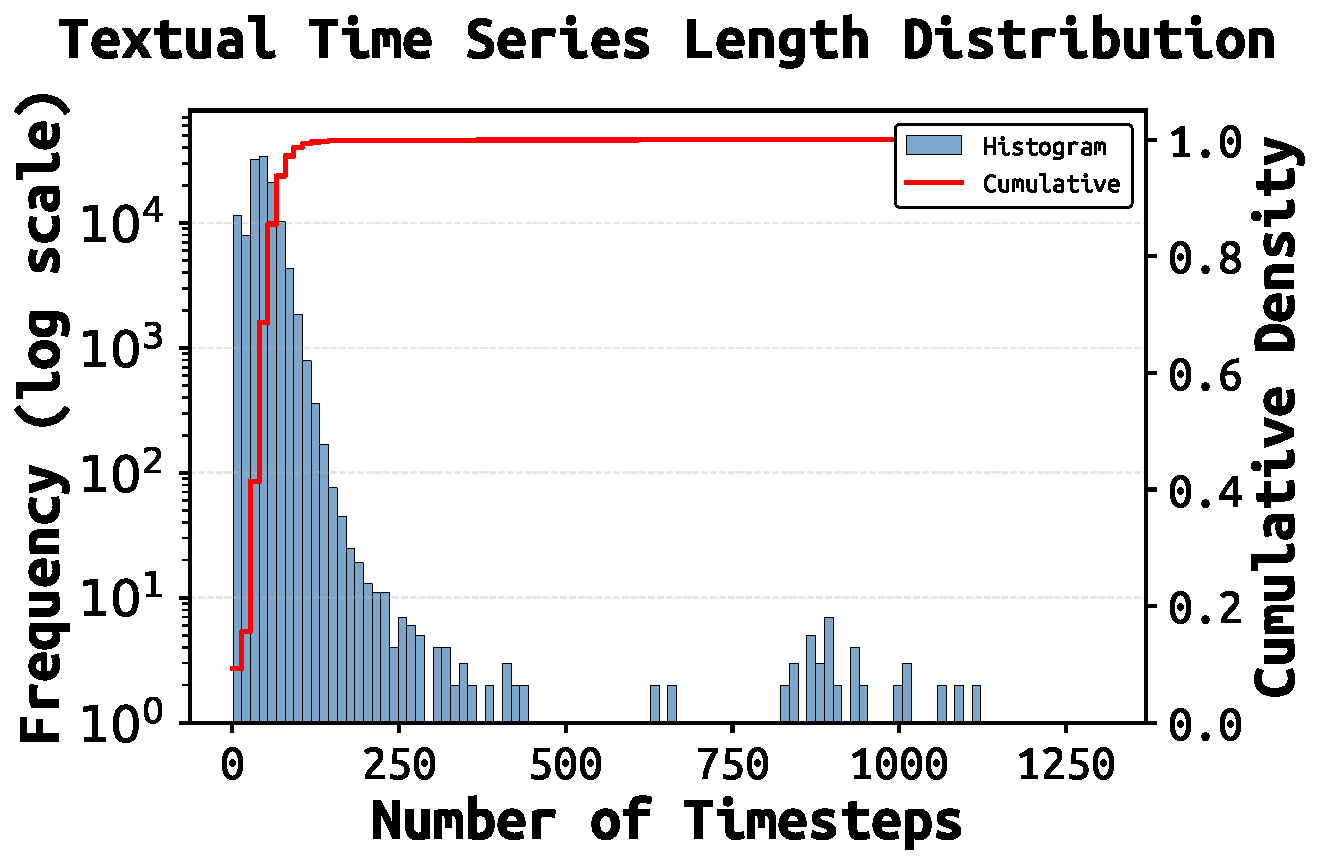
\includegraphics[width=\linewidth]{Chapters/chapter-05/images/Scientific_data/Plots_tables/tts_length_distribution.pdf}
        \ChFivePanelText{(a) Distribution of time series lengths (timesteps) across the dataset.}
    \end{minipage}\hfill
    \begin{minipage}{0.48\textwidth}
        \centering
        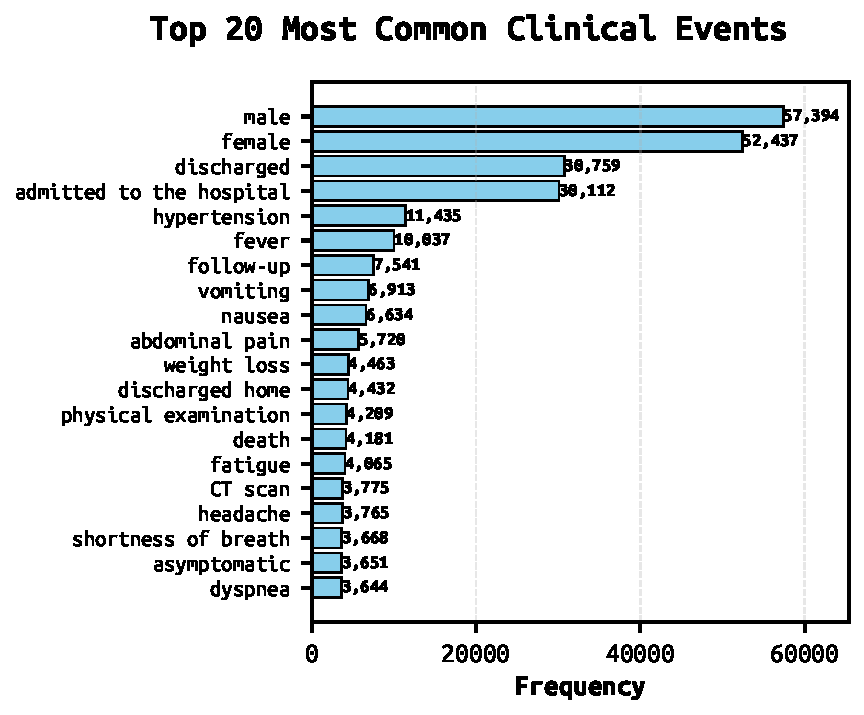
\includegraphics[width=\linewidth]{Chapters/chapter-05/images/Scientific_data/Plots_tables/top_20_common_events.pdf}
        \ChFivePanelText{(b) Most frequently occurring events across all case reports.
        }
    \end{minipage}
    
    
    % \vspace{-7.5mm}

\end{ChFiveFloatBody}
\caption{Overview of textual time series characteristics in PMOA-TTS.}\ChFiveFloatLabel{ch05:fig:tts_stats}
\end{figure}



% !TeX root = ../../../main.tex
\subsubsection{Diagnosis Distribution Analysis}
\label{ch05:diagnosis-distribution-analysis}

To characterize diagnostic coverage, we prompted the LLM to act as an expert physician and list patient-specific diagnoses for each case report. 
The prompt asked the model to extract final diagnostic labels (e.g., ``acne'', ``DRESS syndrome'') rather than isolated clinical findings (e.g., ``rash'', ``leukocytosis''), to place the primary diagnosis first, and to output one diagnosis per line without explanatory text (full prompt in Supplementary Material, Section~\ref{ch05:apd:diagnosis-prompt}).

Free-text diagnoses were then standardized to the Unified Medical Language System (UMLS) using the ScispaCy entity linker (\texttt{en\_core\_sci\_lg}) with the UMLS knowledge base. 
\ChFiveRebuttal{
Each complete extracted diagnosis string was supplied directly to the UMLS candidate generator, with candidate selection designed to avoid fragmentation and improve canonical concept assignment (Supplementary Material, Section~\ref{ch05:apd:umls-mapping}).
}

Figure~\ref{ch05:fig:top_diagnoses} shows the 20 most frequent UMLS-normalized diagnoses in PMOA-TTS.
These are dominated by common cardiometabolic and renal conditions, including hypertensive disease, diabetes mellitus and its subtypes, coronary artery disease, dyslipidemia, and chronic kidney disease.
\ChFiveRebuttal{
Figure~\ref{ch05:fig:diagnoses} characterizes diagnoses represented within PMOA-TTS; it is not an evaluation of diagnostic recognition. Common diagnoses may appear as comorbidities in reports whose primary focus is a rare or atypical presentation.
}

We further examined co-occurrence structure using a clustered heatmap of diagnosis pairs (Figure~\ref{ch05:fig:diagnosis_cooccurrence}).
The heatmap reveals coherent groupings among related conditions, most notably across diabetes variants, as well as broader co-occurrence patterns among cardiovascular, metabolic, and renal diagnoses.
These patterns are consistent with well-established comorbidity relationships (e.g., hypertension with diabetes, or atrial fibrillation with coronary artery disease) and illustrate how the corpus captures clinically meaningful disease constellations.

\ChFiveRebuttal{
To characterize rare-disease representation more directly, we matched UMLS CUIs associated with extracted diagnoses against disorder-level entities in the Orphanet rare-disease nomenclature \citep{lucano2026orphanet} using exact, validated UMLS mappings. After excluding groups and subtypes of disorders and entities designated as inactive, historical, deprecated, obsolete, or non-rare, the reference contained 5,942 Orphanet disorders. Overall, 41{,}775 of 124{,}349 reports (33.6\%) contained at least one extracted diagnosis mapped to an eligible Orphanet disorder, spanning 2,426 distinct ORPHAcodes. Across all extracted diagnoses, 50,299 of 474,075 mappings (10.6\%) matched the Orphanet reference. These statistics characterize rare-disease representation within PMOA-TTS rather than population prevalence.
}


% !TeX root = ../../../main.tex
\begin{figure}[htbp]
\begin{ChFiveFloatBody}

    \centering
    \subfloat[{Most frequent diagnoses.}]{\begin{minipage}[t]{0.39\textwidth}
        \centering
        \raisebox{40pt}{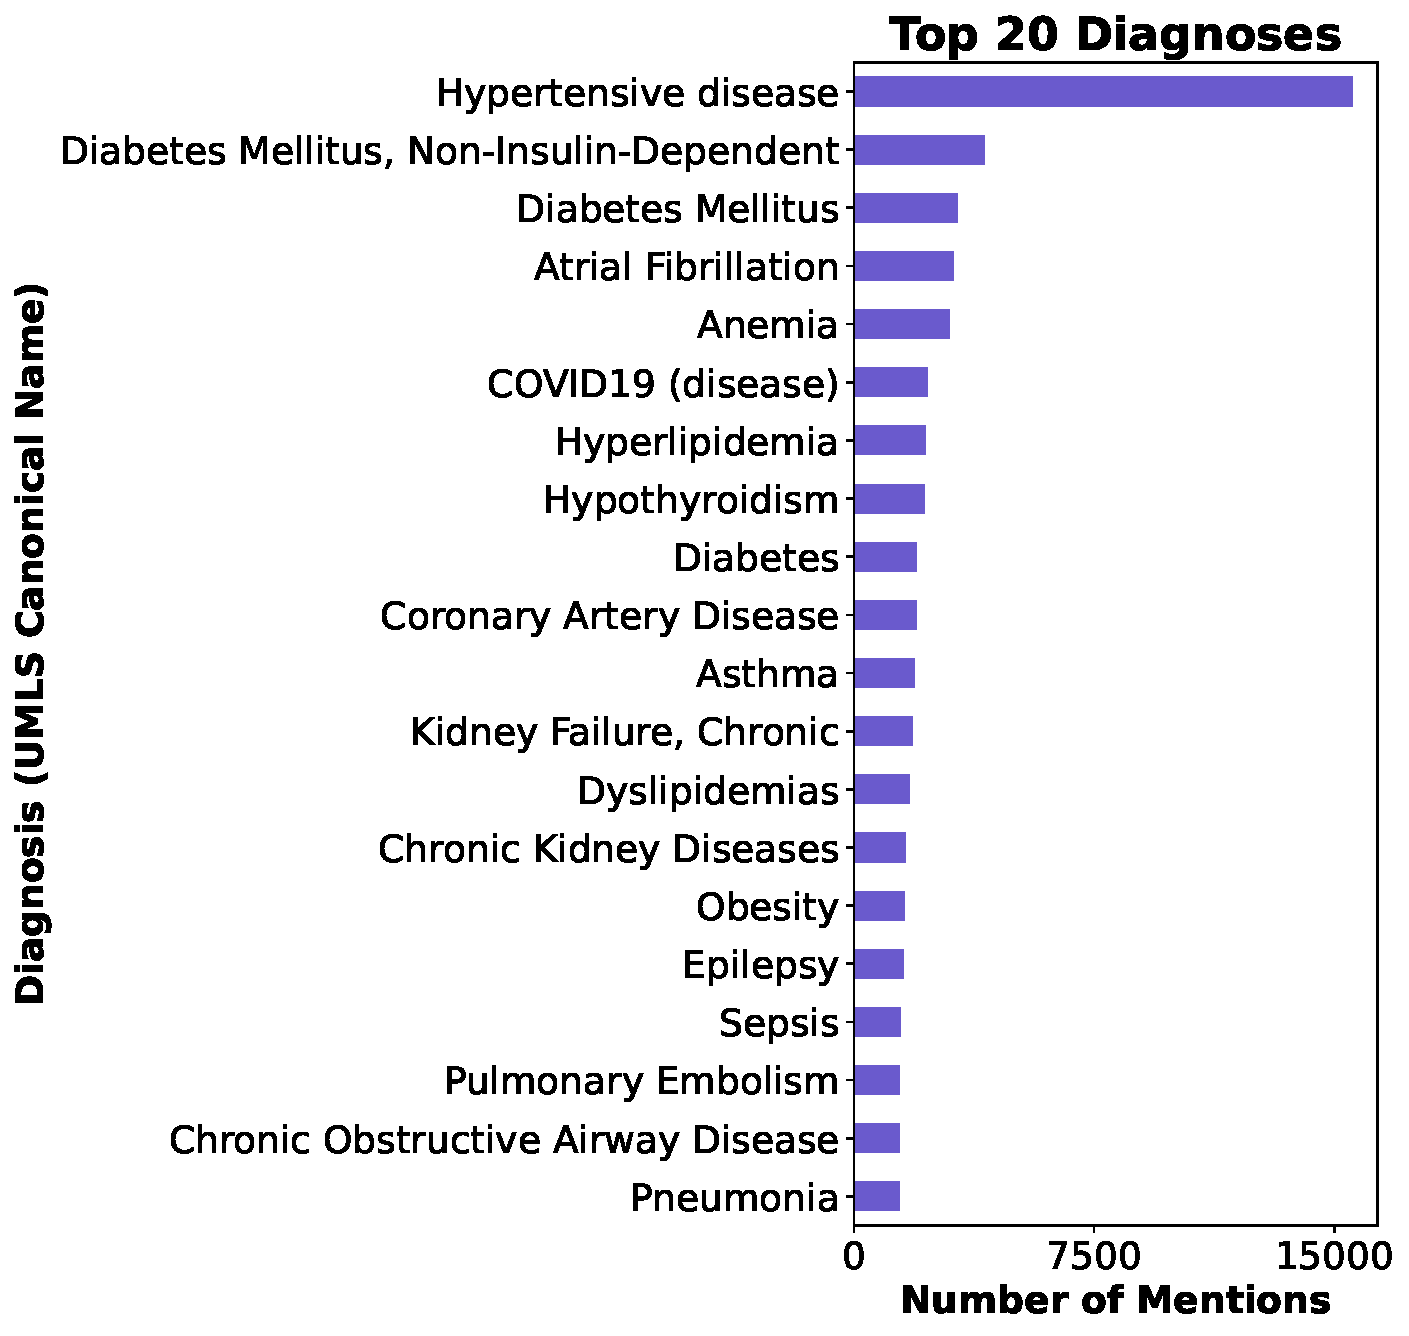
\includegraphics[width=0.99\linewidth]{Chapters/chapter-05/images/Scientific_data/Plots_tables/top_diagnoses_umls_corrected_lexical_tiebreak_paper_ready.pdf}}
        
        \label{ch05:fig:top_diagnoses}
    \end{minipage}}
    \hfill
    \subfloat[{Diagnosis co-occurrence heatmap.}]{\begin{minipage}[t]{0.6\textwidth}
        \centering
        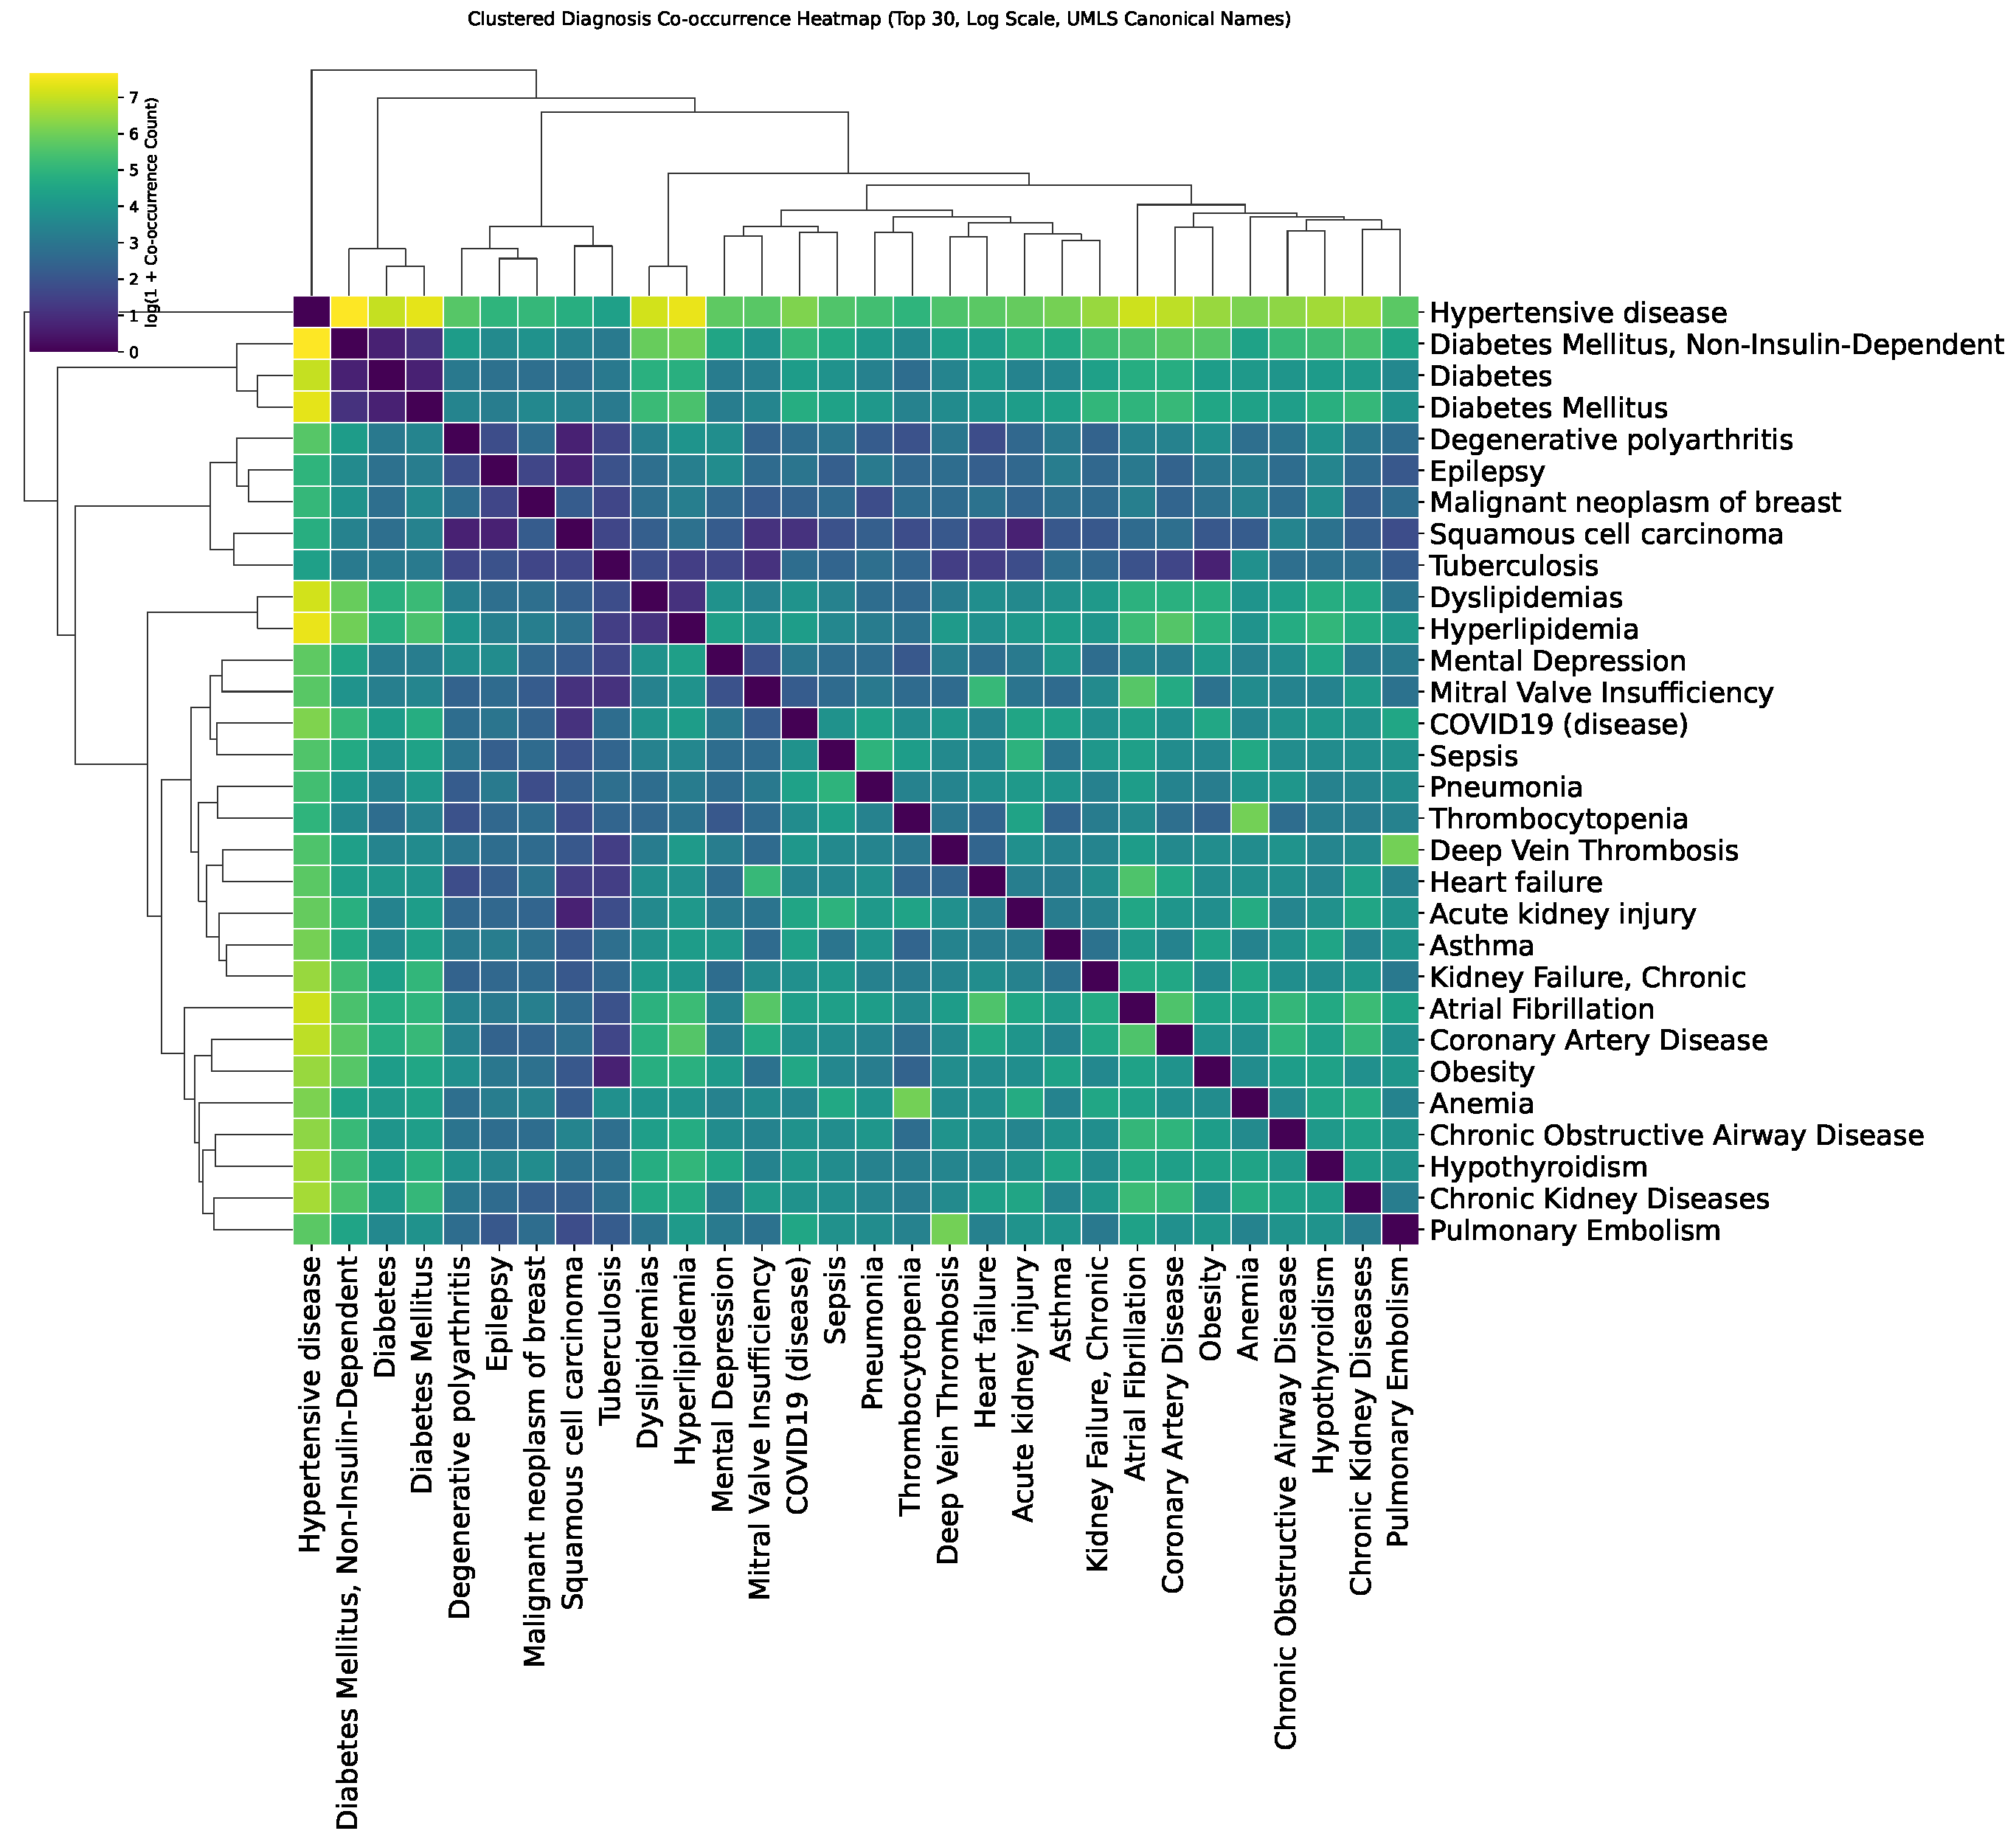
\includegraphics[width=0.99\linewidth]{Chapters/chapter-05/images/Scientific_data/Plots_tables/clustered_cooccurrence_heatmap_top30_corrected_lexical_tiebreak_canonical.pdf}
        
        \label{ch05:fig:diagnosis_cooccurrence}
    \end{minipage}}
    
    
    

\end{ChFiveFloatBody}
\caption{Frequency and co-occurrence patterns of UMLS-normalized diagnoses in PMOA-TTS. (a) The 20 most frequently mentioned diagnoses using canonical UMLS names. (b) Pairwise diagnosis co-occurrence (log-transformed counts) with hierarchical clustering, highlighting groups of frequently co-mentioned conditions.}\ChFiveFloatLabel{ch05:fig:diagnoses}
\end{figure}






% !TeX root = ../../../main.tex
\subsection{Technical Validation}
\label{ch05:sec:technical-validation}


% !TeX root = ../../../main.tex
\ChFiveHeadingOnly
\subsubsection{Case Report Identification Performance}
\label{ch05:sec:case-report-identification-performance}


% !TeX root = ../../../main.tex
\begin{table}[htbp]
\caption{\ChFiveRebuttal{Case-report identification performance by diagnosis and in aggregate on the manually reviewed 100-document evaluation set. Recall is calculated with respect to confirmed single-patient case reports within this evaluation set.}}\ChFiveFloatLabel{ch05:tab:case_report_identification}
\ChFiveTableBodyStart
\begin{ChFiveFloatBody}

\footnotesize
\centering


\begin{tabular}{llcccc}
\toprule
Subset & Diagnosis & Precision & Recall & Accuracy & F1 Score \\
\midrule
\multirow{6}{*}{PubMed metadata} 
    & Atrial Fibrillation & 0.84 & 0.94 & 0.80 & 0.89 \\
    & COVID-19            & 0.94 & 0.89 & 0.85 & 0.92 \\
    & Diabetes            & 0.85 & 1.00 & 0.85 & 0.92 \\
    & Hypertension        & 1.00 & 1.00 & 1.00 & 1.00 \\
    & Sepsis              & 0.95 & 0.95 & 0.90 & 0.95 \\
\cmidrule(lr){2-6}
    & \textbf{All Diagnoses} & \text{0.92} & \textbf{0.96} & \text{0.88} & \text{0.94} \\
\midrule
\multirow{6}{*}{LLM-Pipeline}
    & Atrial Fibrillation & 1.00 & 1.00 & 1.00 & 1.00 \\
    & COVID-19            & 1.00 & 0.89 & 0.90 & 0.94 \\
    & Diabetes            & 1.00 & 0.94 & 0.95 & 0.97 \\
    & Hypertension        & 1.00 & 0.95 & 0.95 & 0.97 \\
    & Sepsis              & 1.00 & 1.00 & 1.00 & 1.00 \\
\cmidrule(lr){2-6}
    & \textbf{All Diagnoses} & \textbf{1.00} & \textbf{0.96} & \textbf{0.96} & \textbf{0.98} \\
\bottomrule
\end{tabular}


\end{ChFiveFloatBody}
\end{table}






Table~\ref{ch05:tab:case_report_identification} reports the performance of the LLM-based pipeline and a PubMed metadata filter for identifying single-patient case reports on the manually reviewed 100-document case-identification evaluation set, evaluated across five diagnostic categories using clinician-assigned labels as reference.
In this evaluation set, the LLM-based pipeline achieved precision of 1.00 across all diagnostic categories and in aggregate, meaning that every document flagged as a single-patient case report by the pipeline was confirmed as such in this sample.
The PubMed metadata filter showed lower and more variable precision, ranging from 0.84 (atrial fibrillation) to 1.00 (hypertension), with an overall precision of 0.92. 
\ChFiveRebuttal{
Within the manually reviewed evaluation set, both methods achieved recall of 0.96, indicating comparable coverage of the confirmed single-patient case reports represented in this set. This quantity is not an estimate of corpus-level sensitivity.
}

Overall accuracy was higher for the LLM-based pipeline (0.96 vs.\ 0.88), largely due to better exclusion of multi-patient or non-case-report articles that were sometimes misclassified by the metadata-based filter.
Performance patterns were consistent across diagnostic subsets, with the LLM pipeline maintaining high F1 scores (0.94--1.00). 
\ChFiveRebuttal{
These results characterize identification performance within the manually reviewed evaluation set; because the set contains documents surfaced by at least one of the two approaches, they do not establish corpus-level sensitivity over PMOA.
}


% !TeX root = ../../../main.tex
\subsubsection{Evaluation of Clinical Textual Time Series Quality}
\label{ch05:sec:evaluation-of-tts-quality}

Using the 200 manually annotated case reports as reference, we evaluated textual time series quality across LLM annotators and runs using event match recall, precision, and F1, temporal concordance (c-index), and AULTC. Table~\ref{ch05:tab:model_comparison} reports mean and standard deviation across runs for seven LLM variants: \texttt{Llama 3.3 70B}, \texttt{DeepSeek-R1}, \texttt{DeepSeek-V3}, \texttt{OpenAI GPT-5}, \texttt{OpenAI O4-mini}, \texttt{OpenAI O3}, and \texttt{OpenAI O1}.

\ChFiveRebuttal{
We additionally evaluated event match precision and F1 to account for model-generated events that were not matched to the manually annotated timeline (Tables~\ref{ch05:tab:model_comparison} and~\ref{ch05:tab:bootstrap_intervals}). Precision varied from 0.756 for GPT-5 to 0.873 for O1, while recall showed the opposite pattern for these models (0.845 for GPT-5 versus 0.637 for O1), illustrating differences in the precision--recall tradeoff across models. F1 ranged from 0.712 to 0.798. Bootstrap 95\% confidence intervals for precision and F1 are reported in Table~\ref{ch05:tab:bootstrap_intervals}. Table~\ref{ch05:tab:model_comparison_lapjv} also includes precision and F1 under the LAPJV-based matching analysis.
}



% !TeX root = ../../../main.tex
\begin{table}[htbp]
\caption{\ChFiveRebuttal{Comparison of models on Event Match Rate (Recall), Event Match Precision, Event Match F1, Concordance, and AULTC with respect to 200 manually annotated case reports across 5 independent runs for each model.}}\ChFiveFloatLabel{ch05:tab:model_comparison}
\ChFiveTableBodyStart
\begin{ChFiveFloatBody}


\footnotesize
\centering
\setlength{\tabcolsep}{3pt}


\begin{tabular}{lccccc}
\hline
\textbf{Model} &
\begin{tabular}{c}\textbf{Event Match}\\\textbf{ Recall}\end{tabular} &
\begin{tabular}{c}\textbf{Event Match}\\\textbf{Precision}\end{tabular} &
\begin{tabular}{c}\textbf{Event Match}\\\textbf{F1}\end{tabular} &
\textbf{Concordance} &
\textbf{AULTC} \\
\hline
\texttt{Llama 3.3 70B}
& 0.673 $\pm$ 0.003
& 0.757 $\pm$ 0.036
& 0.712 $\pm$ 0.015
& 0.846 $\pm$ 0.002
& 0.721 $\pm$ 0.001 \\

\texttt{DeepSeek-R1}
& 0.746 $\pm$ 0.008
& 0.788 $\pm$ 0.006
& 0.766 $\pm$ 0.005
& 0.773 $\pm$ 0.010
& 0.728 $\pm$ 0.004 \\

\texttt{DeepSeek-V3}
& 0.760 $\pm$ 0.004
& 0.796 $\pm$ 0.006
& 0.778 $\pm$ 0.004
& 0.783 $\pm$ 0.007
& 0.731 $\pm$ 0.002 \\

\texttt{OpenAI GPT-5}
& \textbf{0.845 $\pm$ 0.005}
& 0.756 $\pm$ 0.007
& \textbf{0.798 $\pm$ 0.003}
& \textbf{0.902 $\pm$ 0.002}
& 0.722 $\pm$ 0.001 \\

\texttt{OpenAI O4-mini}
& 0.748 $\pm$ 0.019
& 0.814 $\pm$ 0.015
& 0.779 $\pm$ 0.017
& 0.846 $\pm$ 0.006
& \textbf{0.750 $\pm$ 0.002} \\

\texttt{OpenAI O3}
& 0.733 $\pm$ 0.003
& 0.837 $\pm$ 0.003
& 0.782 $\pm$ 0.002
& 0.898 $\pm$ 0.002
& 0.737 $\pm$ 0.003 \\

\texttt{OpenAI O1}
& 0.637 $\pm$ 0.007
& \textbf{0.873 $\pm$ 0.003}
& 0.737 $\pm$ 0.005
& 0.885 $\pm$ 0.002
& 0.732 $\pm$ 0.002 \\
\hline
\end{tabular}


\end{ChFiveFloatBody}
\end{table}




% !TeX root = ../../../main.tex
\begin{table}[htbp]
\caption{\ChFiveRebuttal{Bootstrap 95\% confidence intervals for Event Match Rate (Recall), Event Match Precision, Event Match F1, Concordance, and AULTC across models evaluated on the 200 manually annotated case reports.}}\ChFiveFloatLabel{ch05:tab:bootstrap_intervals}
\ChFiveTableBodyStart
\begin{ChFiveFloatBody}


\footnotesize
\centering
\setlength{\tabcolsep}{3pt}


\begin{tabular}{lccccc}
\hline
\textbf{Model} &
\begin{tabular}{c}\textbf{Event Match}\\\textbf{Recall}\end{tabular} &
\begin{tabular}{c}\textbf{Event Match}\\\textbf{Precision}\end{tabular} &
\begin{tabular}{c}\textbf{Event Match}\\\textbf{F1}\end{tabular} &
\textbf{Concordance} &
\textbf{AULTC} \\
&
\textbf{(95\% CI)} &
\textbf{(95\% CI)} &
\textbf{(95\% CI)} &
\textbf{(95\% CI)} &
\textbf{(95\% CI)} \\
\hline
\texttt{Llama 3.3 70B}
& [0.647, 0.715]
& [0.564, 0.835]
& [0.603, 0.770]
& [0.819, 0.864]
& [0.698, 0.746] \\

\texttt{DeepSeek-R1}
& [0.702, 0.771]
& [0.760, 0.807]
& [0.730, 0.789]
& [0.747, 0.782]
& [0.707, 0.751] \\

\texttt{DeepSeek-V3}
& [0.736, 0.795]
& [0.782, 0.825]
& [0.758, 0.810]
& [0.756, 0.813]
& [0.708, 0.753] \\

\texttt{OpenAI GPT-5}
& [0.812, 0.866]
& [0.751, 0.792]
& [0.780, 0.827]
& [0.889, 0.911]
& [0.702, 0.745] \\

\texttt{OpenAI O4-mini}
& [0.695, 0.764]
& [0.772, 0.828]
& [0.732, 0.795]
& [0.824, 0.868]
& [0.727, 0.772] \\

\texttt{OpenAI O3}
& [0.703, 0.765]
& [0.818, 0.855]
& [0.756, 0.808]
& [0.880, 0.915]
& [0.721, 0.761] \\

\texttt{OpenAI O1}
& [0.612, 0.686]
& [0.864, 0.890]
& [0.717, 0.775]
& [0.869, 0.900]
& [0.712, 0.753] \\
\hline
\end{tabular}


\end{ChFiveFloatBody}
\end{table}



To quantify uncertainty from a complementary perspective, we also performed a bootstrap analysis based on resampling the 200 annotated cases with replacement and recomputing metrics to obtain 95\% confidence intervals. These intervals characterize variability arising from the composition of the reference set, whereas the across-run standard deviations reflect variability in model sampling. The full set of bootstrap intervals is reported in Table~\ref{ch05:tab:bootstrap_intervals}.

% \begin{figure}[!tbp]
% \centering
%     \begin{minipage}[t]{0.242\textwidth}
%     \centering
%     \includegraphics[page=1, width=\linewidth]{Plots_tables/pmoa_updated_man_figs.pdf}
%     \end{minipage}
%     \hfill
%     \begin{minipage}[t]{0.242\textwidth}
%     \centering
%     \includegraphics[page=2, width=\linewidth]{Plots_tables/pmoa_updated_man_figs.pdf}
%     \end{minipage}
%     \hfill
%     \begin{minipage}[t]{0.242\textwidth}
%     \centering
%     \includegraphics[page=3, width=\linewidth]{Plots_tables/pmoa_updated_man_figs.pdf}
%     \end{minipage}
%     \hfill
%     \begin{minipage}[t]{0.242\textwidth}
%     \centering
%     \includegraphics[page=4, width=\linewidth]{Plots_tables/pmoa_updated_man_figs.pdf}
%     \end{minipage}
%     \caption{Comparison of different LLM for extracting temporal clinical events from case reports. From left to right: (\textbf{A}) event match cumulative distribution function, (\textbf{B}) concordance box plots, (\textbf{C}) time discrepancy from manual annotation timestamps among matched events (overall), and (\textbf{D}) time discrepancy disaggregated by clinician annotator timestamp (time from presentation). 
%     %\textcolor{red}{Have same figure for LAPJV?}
%     }
%     \label{fig:tts_evaluation}
%     \vspace{-10pt}
% \end{figure}




% !TeX root = ../../../main.tex
\begin{figure}[htbp]
\begin{ChFiveFloatBody}

\centering

% First row: panels A and B
\begin{minipage}[t]{0.49\linewidth}
    \centering
    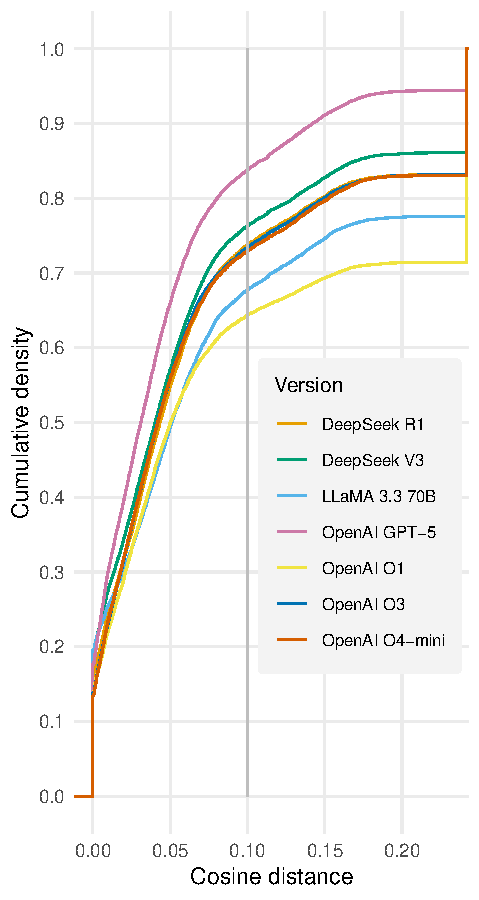
\includegraphics[
        page=1,
        width=0.8\linewidth
    ]{Chapters/chapter-05/images/Plots_tables/pmoa_updated_man_figs.pdf}
\end{minipage}
\hfill
\begin{minipage}[t]{0.49\linewidth}
    \centering
    \includegraphics[
        page=2,
        width=0.8\linewidth
    ]{Chapters/chapter-05/images/Plots_tables/pmoa_updated_man_figs.pdf}
\end{minipage}

\par\medskip

% Second row: panels C and D
\begin{minipage}[t]{0.49\linewidth}
    \centering
    \includegraphics[
        page=3,
        width=0.8\linewidth
    ]{Chapters/chapter-05/images/Plots_tables/pmoa_updated_man_figs.pdf}
\end{minipage}
\hfill
\begin{minipage}[t]{0.49\linewidth}
    \centering
    \includegraphics[
        page=4,
        width=0.8\linewidth
    ]{Chapters/chapter-05/images/Plots_tables/pmoa_updated_man_figs.pdf}
\end{minipage}





\end{ChFiveFloatBody}
\caption{
Comparison of different LLMs for extracting temporal clinical events
from case reports:
(\textbf{A}) cumulative distribution of event-matching cosine distances;
(\textbf{B}) temporal-concordance box plots;
(\textbf{C}) timestamp discrepancies between model-generated and manual
annotations among semantically matched events; and
(\textbf{D}) timestamp discrepancies stratified by the clinician-annotated
time relative to presentation.
}\ChFiveFloatLabel{ch05:fig:tts_evaluation}
\end{figure}



\paragraph{Text Event Match Performance}
\label{ch05:sec:text-event-match-performance}
Figure~\ref{ch05:fig:tts_evaluation} (A) shows the cumulative distributions of cosine distances between model-generated and reference event descriptions, with a threshold of 0.1 used to define a successful semantic match. At this threshold, 
\ChFiveRebuttal{
\texttt{GPT-5} had the highest mean event-recall point estimate (0.845), followed by \texttt{DeepSeek-V3} (0.760), \texttt{O4-mini} (0.748), and \texttt{DeepSeek-R1} (0.746). \texttt{O3} and \texttt{Llama 3.3 70B} had mean recall values of 0.733 and 0.673, respectively, while \texttt{O1} had the lowest mean recall (0.637). These point estimates show variation across models in the proportion of manually annotated clinical events recovered under the selected semantic-matching threshold.
}
% \ChFiveRebuttal{
% \texttt{GPT-5} achieved the highest mean event recall (0.845), followed by \texttt{DeepSeek-V3} (0.760), \texttt{O4-mini} (0.748), and \texttt{DeepSeek-R1} (0.746). \texttt{O3} and \texttt{Llama 3.3 70B} achieved lower recall of 0.733 and 0.673, respectively, while \texttt{O1} had the lowest recall (0.637). These results indicate meaningful differences across models in the proportion of manually annotated clinical events recovered under the selected semantic-matching threshold.
% }

\paragraph{Temporal Ordering Performance}
\label{ch05:sec:temporal-ordering-performance}

Using the same similarity threshold to identify matched events, temporal ordering accuracy was evaluated with the concordance index (c-index). As shown in Figure~\ref{ch05:fig:tts_evaluation} (B),
\ChFiveRebuttal{
\texttt{GPT-5} had the highest mean concordance point estimate (0.902), followed closely by \texttt{O3} (0.898) and \texttt{O1} (0.885). \texttt{Llama 3.3 70B} and \texttt{O4-mini} both had mean concordance of 0.846, while \texttt{DeepSeek-V3} and \texttt{DeepSeek-R1} had mean concordance of 0.783 and 0.773, respectively. However, the bootstrap 95\% confidence intervals for the leading models overlapped. We therefore interpret the ordering of the mean estimates descriptively and do not consider these results evidence that one model was statistically superior in temporal ordering.
The differences between event recall and concordance across models illustrate that these metrics capture distinct aspects of timeline quality. For example, \texttt{O1} had the lowest event recall but relatively high concordance among the events that were successfully matched.
}
% \ChFiveRebuttal{\texttt{GPT-5} achieved the highest mean concordance (0.902), closely followed by \texttt{O3} (0.898) and \texttt{O1} (0.885). \texttt{Llama 3.3 70B} and \texttt{O4-mini} both achieved concordance of 0.846, while \texttt{DeepSeek-V3} and \texttt{DeepSeek-R1} had lower concordance of 0.783 and 0.773, respectively. The differences between event recall and concordance across models illustrate that event recovery and temporal ordering capture distinct aspects of timeline quality. For example, \texttt{O1} had the lowest event recall but relatively high concordance among the events that were successfully matched.}
This contrast highlights that models that align fewer but clearer events may achieve high ordering scores, whereas models with broader coverage face a more challenging ordering task.


\paragraph{Time Discrepancy Analysis}
\label{ch05:sec:time-descrepancy-analysis}
Figure~\ref{ch05:fig:tts_evaluation} (C, D) presents cumulative distributions of log-scaled time discrepancies between predicted and reference timestamps for semantically matched events. 
\ChFiveRebuttal{
\texttt{O4-mini} had the highest mean AULTC point estimate (0.750), followed by \texttt{O3} (0.737). \texttt{O1}, \texttt{DeepSeek-V3}, and \texttt{DeepSeek-R1} had similar intermediate mean values of 0.732, 0.731, and 0.728, respectively, while \texttt{GPT-5} (0.722) and \texttt{Llama 3.3 70B} (0.721) had the lowest mean AULTC values. However, the bootstrap 95\% confidence intervals overlapped across several models. We therefore treat this ordering as descriptive and do not interpret the higher mean for \texttt{O4-mini} as evidence of statistically distinct superiority in timestamp accuracy.
The variation in mean AULTC was smaller than the variation observed for event recall and temporal concordance. The interval-stratified analysis in Figure~\ref{ch05:fig:tts_evaluation} (D) further shows how timestamp accuracy varies with temporal distance from the admission reference time.
}
% \ChFiveRebuttal{
% \texttt{O4-mini} achieved the highest mean AULTC (0.750), followed by \texttt{O3} (0.737). \texttt{O1}, \texttt{DeepSeek-V3}, and \texttt{DeepSeek-R1} achieved similar intermediate values of 0.732, 0.731, and 0.728, respectively, while \texttt{GPT-5} (0.722) and \texttt{Llama 3.3 70B} (0.721) had the lowest mean AULTC values. 
% Notably, the spread in AULTC performance is less pronounced than that observed for the event match rate and concordance.
% The interval-stratified analysis in Figure~\ref{ch05:fig:tts_evaluation} (D) further shows how timestamp accuracy varies with temporal distance from the admission reference time.
% }

Taken together, these results show that semantic matching, temporal ordering, and timestamp accuracy provide complementary views of textual time series quality. Because the leading mean estimates differ across metrics and their bootstrap confidence intervals frequently overlap, we do not designate a single best-performing model.

\paragraph{Timestamp Provenance Audit}
\label{ch05:sec:timestamp-provenance-audit}

\ChFiveRebuttal{
The production TTS schema stores a single timestamp for each extracted event and does not distinguish whether the timestamp is directly supported by temporal information in the source text or inferred from narrative context. Because this provenance was not retained during full-corpus generation, we conducted a targeted audit of the 200 evaluation reports using GPT-5. We retained the original event-time extraction task while adding a binary \emph{known} indicator for each event. \emph{known=1} was assigned when the timestamp was anchored by admission/presentation or directly supported by an absolute or relative temporal expression in the source text; \emph{known=0} was assigned when the timestamp was inferred from narrative context or clinical judgment.
}

\ChFiveRebuttal{
Across 11,618 extracted events, 6,314 (54.35\%) timestamps were text-supported or directly anchored (\emph{known=1}), while 5,304 (45.65\%) were inferred (\emph{known=0}). At the case level, the median proportion of text-supported timestamps was 53.29\% (IQR: 31.58\%--75.52\%). Thus, while a slight majority of timestamps could be tied directly to temporal evidence under this definition, temporal imputation accounts for a considerable fraction of the generated timelines. This audit is limited to GPT-5 outputs on the evaluation sample and does not provide provenance annotations for the full corpus or establish that the observed proportions generalize to other extraction models.
}

\paragraph{Inter-annotator agreement on a GLP1-RA subset}
\label{ch05:glp_iaa}

\ChFiveRebuttal{To contextualize agreement with the single-expert reference set, we also analyzed a separate 140-case report subset of PMOA-TTS involving patients who took GLP-1 RA (Glucagon-like Peptide Receptor Agonists) medications. Two clinically trained annotators independently constructed event-time timelines for this subset using the same annotation framework. Using Annotator 1 as the reference and the same matching and temporal metrics used for the model evaluation, Annotator 2 achieved an event match rate of 0.811, temporal concordance of 0.798, and AULTC of 0.702.}


% !TeX root = ../../../main.tex
\subsubsection{Additional Sensitivity Analyses}
\label{ch05:sec:additional-sensitivity-analyses}

\ChFiveHeadingOnly
\paragraph{Varying the Event Match Distance Threshold}

We conducted sensitivity analyses to assess robustness with respect to the event match threshold.
As expected, stricter thresholds produce fewer but cleaner matches, while more permissive thresholds increase coverage at the expense of noisier ordering and timing.
Varying the cosine distance threshold from \ChFiveRebuttal{0.01 to 0.50 (in increments of 0.01 for both the recursive and LAPJV matching analyses)}, we observed corresponding shifts in event match recall, concordance, and AULTC.
A threshold of 0.10 was chosen based on manual review of \texttt{Llama 3.3 70B Instruct} and \texttt{O1} outputs.
The resulting trade-offs are summarized in Figure~\ref{ch05:fig:threshold_tradeoff_greedy}.



Similarly, LAPJV preserves high event match rates at low thresholds across models and exhibits a smooth trade-off between coverage and temporal accuracy (Supplementary Material, Section \ref{ch05:apd:lapjv-matching} Figure~\ref{ch05:fig:threshold_tradeoff_LAPJV}).
The resulting operating points are highly comparable to those obtained using the recursive matching heuristic.
In particular, the heuristic matcher yields slightly stronger concordance near the elbow of the trade-off curve, while LAPJV achieves marginally higher AULTC values, reflecting improved timestamp alignment under global assignment.
Overall, both strategies lead to consistent qualitative conclusions.

\ChFiveRebuttal{For both Figure~\ref{ch05:fig:threshold_tradeoff_greedy} and Figure~\ref{ch05:fig:threshold_tradeoff_LAPJV}, model trajectories change smoothly in the neighborhood of 0.1, but the rank
order is not invariant across the full threshold range, particularly for AULTC where several curves are close or cross.
We therefore interpret the curves as coverage-versus-temporal-accuracy trade-offs rather than evidence of one
threshold-independent winner.}


\paragraph{Sensitivity to Parts of the LLM Prompt Being Changed}
We conducted sensitivity analyses to assess how different components of the extraction prompt affect timeline quality (Supplementary Material, Section~\ref{ch05:apd:sensitivity-llm-prompt}).
Structured prompts that include explicit temporal instructions (e.g., Interval and Interval+Type) consistently improved semantic alignment, temporal ordering, and timestamp accuracy.
In contrast, removing role framing or conjunction expansion led to modest degradation, and Zero-shot prompting performed substantially worse across all metrics.
These results highlight that prompt design plays an important role in guiding LLMs to produce high-quality temporal annotations (Figure~\ref{ch05:fig:prompt_ablation}).



% !TeX root = ../../../main.tex
\begin{figure}[htbp]
\begin{ChFiveFloatBody}
\centering
        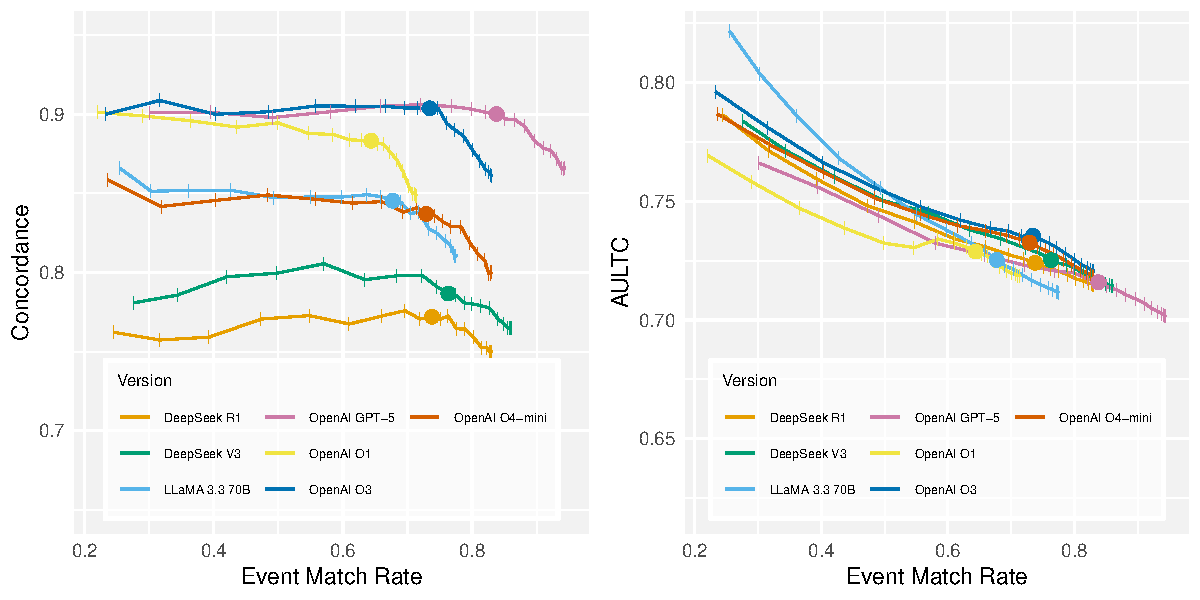
\includegraphics[width=\linewidth]{Chapters/chapter-05/images/Scientific_data/Plots_tables/event_match_vs_metrics_updated.pdf}

    
    
    

\end{ChFiveFloatBody}
\caption{Concordance and AULTC by event match rate for recursive matching heuristic. Solid circle ($\bullet$) represents threshold of 0.1, with ticks (|) indicating 0.01 increments of the threshold in [0.01, 0.50].
    }\ChFiveFloatLabel{ch05:fig:threshold_tradeoff_greedy}
\end{figure}





\paragraph{Inter-LLM comparison of temporal annotations}
Finally, we qualitatively compared temporal annotations produced by several LLMs on a representative case report to illustrate characteristic differences in event extraction and timestamping (Supplementary Material, Section~\ref{ch05:apd:inter-llm-comparison}, Figure~\ref{ch05:fig:tts_evaluation}).
While all models recovered the major clinical trajectory and preserved temporal polarity, they varied in
event granularity, paraphrasing, and long-range temporal normalization.
These differences complement the aggregate quantitative results and highlight the impact of model behavior on the structure of extracted timelines.
Common model-specific error patterns, such as granularity variation, duplicate events, and differences in temporal normalization, are summarized in the Supplementary Material, Section~\ref{ch05:apd:inter-llm-comparison}, Table~\ref{ch05:tab:error_taxonomy}.

\paragraph{Validation of Structured Fields}
\label{ch05:sec:structured-field-validation}

\ChFiveRebuttal{
We manually validated the structured fields on 88 confirmed case reports of \texttt{case\_study\_100} split. Across 264 demographic fields, 247 were correct (93.6\%): age accuracy was 95.5\% (84/88), sex accuracy was 97.7\% (86/88), and ethnicity accuracy was 87.5\% (77/88). Of 517 extracted diagnosis entries, 505 were supported by the source report, corresponding to 97.7\% precision. After revising the UMLS-linking procedure, 478/517 diagnosis mappings (92.46\%) were judged acceptable and 39/517 (7.54\%) incorrect.
}

\ChFiveRebuttal{
Demographic errors were concentrated in missing or malformed values; diagnosis errors primarily reflected family history, excluded differentials, or hypothetical complications assigned to the patient. UMLS errors most often involved an inappropriate semantic type or an overly generic concept.
}



% !TeX root = ../../../main.tex
\subsubsection{Limitations and Future Directions}
\label{ch05:sec:limitations-and-future-directions}

Our temporal annotation pipeline has several important limitations. 
\ChFiveRebuttal{
First, because published case reports preferentially describe unusual, severe, or diagnostically complex presentations, PMOA-TTS is not representative of routine clinical populations. Analyses of diagnosis frequencies should therefore be interpreted as descriptions of the corpus rather than estimates of disease prevalence.
}
\ChFiveRebuttal{
Demographic fields may contain unsupported inferences, missing-value errors, and category-mapping errors and should not be used as verified patient attributes without source-level review.
}
At the same time, we should still note that case reports offer rich, temporally structured narratives with explicit clinical rationale, making them a useful testbed for developing and stress-testing textual time series methods.
Our LLM-based framework is designed to be reusable and, in ongoing work, is being adapted to corpora such as MIMIC-IV discharge summaries for future dataset releases.

Second, we model events as minimally modified text spans aligned to the source narrative.
This design choice preserves interpretability and facilitates direct comparison with the underlying text but relies on embedding-based matching for evaluation and does not normalize event content to standard clinical ontologies such as UMLS. \ChFiveRebuttal{The free-text representation introduces lexical variation across reports. Synonym-aware retrieval and event-level mappings to controlled vocabularies may be added as downstream views of the data, but the source-faithful span should be retained so that normalization does not remove clinically important context or modifiers.}

Third, representing time with single relative points simplifies annotation and downstream use but cannot fully capture durations or complex temporal relations (e.g., overlapping intervals or recurrent events).

Fourth, our one-to-one recursive event matching strategy emphasizes temporal consistency at the expense of recall, especially when the same clinical concept is expressed multiple times or in conjunctive form.
Alternative matching formulations (e.g., many-to-many or cluster-based matching) could improve coverage but would require more elaborate evaluation protocols. 

These limitations point to several directions for future work, including ontology-aware event normalization, richer temporal representations (intervals and uncertainty), improved matching algorithms, and extension of the pipeline to diverse EHR-derived note types.


    
    

    
    



% !TeX root = ../../../main.tex
\begin{figure}[htbp]
\begin{ChFiveFloatBody}

\centering
    \begin{minipage}[t]{0.242\textwidth}
    \centering
    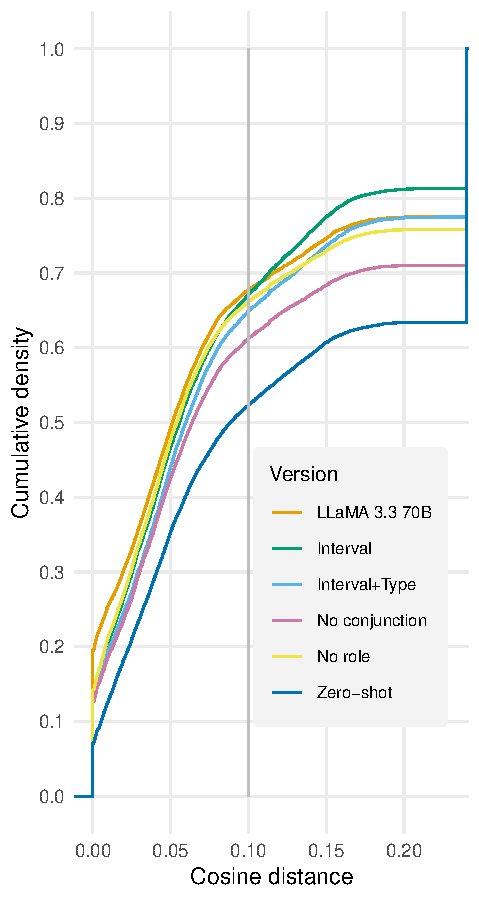
\includegraphics[page=1, width=\linewidth]{Chapters/chapter-05/images/Plots_tables/prompt_ablation_updated_figure.pdf}
    \end{minipage}
    \hfill
    \begin{minipage}[t]{0.242\textwidth}
    \centering
    \includegraphics[page=2, width=\linewidth]{Chapters/chapter-05/images/Plots_tables/prompt_ablation_updated_figure.pdf}
    \end{minipage}
    \hfill
    \begin{minipage}[t]{0.242\textwidth}
    \centering
    \includegraphics[page=3, width=\linewidth]{Chapters/chapter-05/images/Plots_tables/prompt_ablation_updated_figure.pdf}
    \end{minipage}
    \hfill
    \begin{minipage}[t]{0.242\textwidth}
    \centering
    \includegraphics[page=4, width=\linewidth]{Chapters/chapter-05/images/Plots_tables/prompt_ablation_updated_figure.pdf}
    \end{minipage}
    
    
    

\end{ChFiveFloatBody}
\caption{Comparison of \texttt{Llama 3.3 70B} prompt ablation and variant methods for extracting temporal clinical events from case reports. From left to right: (\textbf{A}) event match cumulative distribution function, (\textbf{B}) concordance box plots, (\textbf{C}) time discrepancy from manual annotation timestamps among matched events (overall), and (\textbf{D}) time discrepancy disaggregated by clinician annotator timestamp (time from presentation).}\ChFiveFloatLabel{ch05:fig:prompt_ablation}
\end{figure}















% % !TeX root = ../../../main.tex
\subsection{Usage Notes}
\label{ch05:sec:usage-notes}

Our full codebase, including preprocessing scripts, prompt templates, and evaluation pipelines,
is available at: \url{https://github.com/jcweiss2/pmoa_tts}.
Each subdirectory contains its own README.md with detailed instructions and information.
Here is the repository structure
\begin{itemize}
    \item \texttt{make\_tts}: Scripts and notebooks for constructing the PMOA-TTS dataset from case reports.
    \item \texttt{TTS\_evaluation}: Evaluation scripts assessing the quality of the extracted timelines.
\end{itemize}

\noindent Here are step-by-step directions on how to use the dataset

\begin{enumerate}

\item \textbf{Clone the repository:}

{\small
\begin{verbatim}
    git clone https://github.com/jcweiss2/pmoa_tts.git
    cd pmoa_tts
\end{verbatim}
}

\item \textbf{Set up the environment:}

\noindent Ensure you have Python 3.10 or higher installed. It's recommended to use a virtual environment.

{\small
\begin{verbatim}
    conda create -n pmoa_tts python=3.10
    conda activate pmoa_tts
    conda install pandas scikit-learn numpy tensorboard -c conda-forge
    conda install pytorch torchvision torchaudio -c pytorch
    pip install transformers
    pip install argparse
    conda install jupyter -c conda-forge
    pip install sentencepiece
\end{verbatim}
}

\item \textbf{Access the PMOA-TTS dataset.} The dataset is available on Hugging Face.
You can download it using the \texttt{datasets} library.

{\small
\begin{verbatim}
    from datasets import load_dataset
    dataset = load_dataset("snoroozi/pmoa-tts")
\end{verbatim}
}

\end{enumerate}

\ChFiveParagraph{Responsible reuse and cautions}

The release and use of PMOA–TTS raise important considerations.
Although LLMs achieve strong performance, they may still generate inaccurate or hallucinated outputs, and any downstream use of these annotations without further validation could introduce bias or error.
The extraction of structured diagnoses, demographics, and clinical events from public text—though non-identifiable—could also lead to misinterpretation or reinforce historical biases if not handled carefully.
Furthermore, while the dataset is intended for research, there is a risk of misapplication in high-stakes clinical settings without expert oversight.
Lastly, the stylistic and structural differences between case reports and real-world EHR notes may limit the generalizability of findings derived from PMOA–TTS.
These limitations underscore the importance of using the corpus responsibly, with clear reporting of model limitations and appropriate safeguards when applied in downstream tasks.



% % !TeX root = ../../../main.tex
\ChFiveStarSection{Code availability}\label{ch05:sec:data_availability}
In line with the philosophy of reproducible research, all codes used in this paper, including those for data preprocessing and technical validation, are accessible at \url{https://github.com/jcweiss2/pmoa_tts}. The usage instructions and parameter settings for all codes can be found at this link.


% % !TeX root = ../../../main.tex
\ChFiveStarSection{Funding}

This research was supported in part by the Division of Intramural Research (DIR) of the National Library of Medicine (NLM), National Institutes of Health.
This work utilized the computational resources of the NIH HPC Biowulf cluster.
S. N. was supported by Carnegie Mellon University TCS Presidential Fellowship, and Natural Sciences and Engineering Research Council of Canada (NSERC) PGS-D award.
S.N was also supported in part by an appointment to the National Library of Medicine Research Participation Program administered by the Oak Ridge Institute for Science and Education (ORISE) through an interagency agreement between the U.S. Department of Energy (DOE) and the National Library of Medicine, National Institutes of Health.
ORISE is managed by ORAU under DOE contract number DE-SC0014664.
All opinions expressed in this paper are the authors’ and do not necessarily reflect the policies and views of NIH, NLM, DOE, or ORAU/ORISE.



% % !TeX root = ../../../main.tex
\ChFiveStarSection{Author contributions}

These authors contributed equally: Shahriar Noroozizadeh (S.N.) and Sayantan Kumar (S.K.).
S.N. and S.K. implemented the pipeline, ran all experiments, curated the data, performed analyses and visualizations, and drafted/revised the manuscript.
Jeremy C. Weiss (J.C.W.) conceived the study, guided methodology, contributed to experiments, supervised the project, and secured funding.
George Chen (G.C.) contributed to technical discussions and manuscript review.
All authors approved the final manuscript.



\clearpage
\endgroup
